\documentclass[sigconf]{acmart}

\usepackage{etex}
\usepackage{flushend}

\usepackage{booktabs} % For formal tables
\usepackage{blindtext} % Package to generate dummy text throughout this template 
\usepackage{lettrine} % The lettrine is the first enlarged letter at the beginning of the text
\usepackage{listings} % para formatar código-fonte (ex. em Java)

\usepackage[utf8]{inputenc}
\usepackage[brazil]{babel}

\usepackage{enumitem} 
\setlist[itemize]{noitemsep}
%\setlist[itemize]{leftmargin=*}
\setlist[enumerate]{itemsep=0mm}


\usepackage{multirow}

\renewcommand{\lstlistingname}{Código-Fonte}
\renewcommand{\tablename}{Tabela}
\renewcommand{\figurename}{Figura}

\newcommand{\remark}[2]{{\small\textsl{\textbf{#1: #2}}}}
\newcommand{\mau}[1]{\remark{Maurício:}{\textcolor{red}{#1}}} 


\definecolor{Maroon}{rgb}{0.5,0,0}
\definecolor{darkgreen}{rgb}{0,0.5,0}
\definecolor{eclipseBlue}{RGB}{42,0.0,255}
\definecolor{eclipseGreen}{RGB}{63,127,95}
\definecolor{eclipsePurple}{RGB}{127,0,85}

\lstdefinelanguage{XML_android}
{
  morestring=[b]",
  moredelim=[s][\color{Maroon}]{<}{\ },
  moredelim=[s][\color{Maroon}]{</}{>},
  moredelim=[l][\color{Maroon}]{/>},
  moredelim=[l][\color{Maroon}]{>},
  morecomment=[s]{<?}{?>},
  morecomment=[s]{<!--}{-->},
  commentstyle=\color{darkgreen},
  stringstyle=\color{blue},
  identifierstyle=\color{red}
}

\lstdefinelanguage{XML_SYNTAX}{%
    morekeywords={id},
    alsoletter=-,
    morestring=[b]",
    stringstyle=\color[rgb]{0,0,1},
    morecomment=[s]{<?}{?>},
    morecomment=[s]{<!--}{-->},
    morecomment=[s]{<!}{>},
    commentstyle=\color{darkgreen},
    moredelim=[s][\color{black}]{![}{]]},
    moredelim=*[s][\color{Maroon}]{<}{>},
    % keywordstyle=\color{red}
}

% Set Language
\lstset{
  language={XML},
  basicstyle=\small\ttfamily, % Global Code Style
  captionpos=b, % Position of the Caption (t for top, b for bottom)
  extendedchars=true, % Allows 256 instead of 128 ASCII characters
  tabsize=2, % number of spaces indented when discovering a tab 
  columns=fixed, % make all characters equal width
  keepspaces=true, % does not ignore spaces to fit width, convert tabs to spaces
  showstringspaces=false, % lets spaces in strings appear as real spaces
  breaklines=true, % wrap lines if they don't fit
  frame=trbl, % draw a frame at the top, right, left and bottom of the listing
  % frameround=tttt, % make the frame round at all four corners
  % framesep=4pt, % quarter circle size of the round corners
  % numbers=left, % show line numbers at the left
  % numberstyle=\tiny\ttfamily, % style of the line numbers
  % commentstyle=\color{eclipseGreen}, % style of comments
  % keywordstyle=\color{eclipsePurple}, % style of keywords
  % stringstyle=\color{eclipseBlue}, % style of strings
  stringstyle=\color[rgb]{0,0,0},
}


\renewcommand{\arraystretch}{1.3}


% Pacotes de Gráficos
\usepackage{tikz} \usetikzlibrary{calc,plotmarks}  
\usepackage{pgfplots}
\usepackage{graphicx}
\usepackage{subcaption}


\graphicspath{{./images/}} % caminho das figuras (recomendável)

% Copyright
%\setcopyright{none}
%\setcopyright{acmcopyright}
%\setcopyright{acmlicensed}
\setcopyright{rightsretained}
%\setcopyright{usgov}
%\setcopyright{usgovmixed}
%\setcopyright{cagov}
%\setcopyright{cagovmixed}


% DOI
\acmDOI{10.475/123_4}

% ISBN
\acmISBN{123-4567-24-567/08/06}

%Conference
\acmConference[SBES'17]{SBES 2017: 31st Brazilian Symposium on Software Engineering}{Setembro 2017}{Fortaleza, Ceará Brasil} 
\acmYear{2017}
\copyrightyear{2017}

\acmPrice{15.00}

% \overfullrule=2cm % marca todas as linhas que estão "vazando"

\usepackage[T1]{fontenc}
\hyphenation{prá-ti-cas}
\hyphenation{prá-ti-ca}
\hyphenation{más}
\hyphenation{co-mo}

\begin{document}

% \title{Sobre a Percepção dos Desenvolvedores Android em Relação aos Maus Cheiros de Código}
\title{Maus cheiros de código em aplicativos Android: Um estudo sobre a percepção dos desenvolvedores}
% \titlenote{Produces the permission block, and copyright information}
% \subtitle{Extended Abstract}
% \subtitlenote{The full version of the author's guide is available as
%   \texttt{acmart.pdf} document}


\author{Suelen G. Carvalho}
% \authornote{Dr.~Trovato insisted his name be first.}
% \orcid{1234-5678-9012}
\affiliation{
  \institution{Universidade de São Paulo}
  \streetaddress{Rua do Matão, 1010}
  \city{São Paulo} 
  \state{SP} 
  \postcode{05508-090}
}
\email{suelengc@ime.usp.br}

\author{Marco Aurélio Gerosa}
\affiliation{
  \institution{Northern Arizona University}
  \streetaddress{E Runke Dr}
  \city{Flagstaff} 
  \state{Arizona} 
  \postcode{86011}
}
\email{marco.gerosa@nau.edu}

\author{Maurício Aniche}
\affiliation{
  \institution{Delft University of Technology}
  \streetaddress{Mekelweg 2}
  \city{Delft} 
  \state{The Netherlands} 
  \postcode{2628 CD}
}
\email{m.f.aniche@tudelft.nl}

% The default list of authors is too long for headers}
% \renewcommand{\shortauthors}{B. Trovato et al.}


\begin{abstract}
Android is the most widely used mobile operating system with 83\% of the world market and more than 2 million applications available in the official store. Android applications have been made complex software projects that need to be quickly developed and regularly evolved to meet the requirements of users. This context can lead to bad code design choices, known as code smells, that can become anomalies that degrade project quality, making it difficult to maintain. Consequently, software developers need to identify problematic code snippets in order to have a code base that favors maintenance and evolution. For this, developers often make use of techniques to detect code smells. Although there are already several code smells cataloged, such as God Class and Long Method, they do not take into account the nature of the project. Researches demonstrated that different platforms, languages and frameworks present specific code quality metrics. Android projects have specific characteristics, such as a directory that stores all the resources used and a class that tends to accumulate various responsibilities. Research on Android are still few. In this dissertation we aim to identify, validate and document code smells related with presentation layer of Android, where the greatest differences are found when compared to traditional projects. In other works on Android, were identified code smells related to safety, intelligent features or somehow impact the experience or user expectation consumption. Unlike them, our proposal is to catalog code smells Android that influence the quality of the code. With this, developers will have another resource for producing quality code.

\noindent \textbf{Keywords:} android, code smells, code quality, code anomalies, code metrics.
\end{abstract}

%
% The code below should be generated by the tool at
% http://dl.acm.org/ccs.cfm
% Please copy and paste the code instead of the example below. 
%
\begin{CCSXML}
<ccs2012>
 <concept>
  <concept_id>10010520.10010553.10010562</concept_id>
  <concept_desc>Computer systems organization~Embedded systems</concept_desc>
  <concept_significance>500</concept_significance>
 </concept>
 <concept>
  <concept_id>10010520.10010575.10010755</concept_id>
  <concept_desc>Computer systems organization~Redundancy</concept_desc>
  <concept_significance>300</concept_significance>
 </concept>
 <concept>
  <concept_id>10010520.10010553.10010554</concept_id>
  <concept_desc>Computer systems organization~Robotics</concept_desc>
  <concept_significance>100</concept_significance>
 </concept>
 <concept>
  <concept_id>10003033.10003083.10003095</concept_id>
  <concept_desc>Networks~Network reliability</concept_desc>
  <concept_significance>100</concept_significance>
 </concept>
</ccs2012>  
\end{CCSXML}

% \ccsdesc[500]{Computer systems organization~Embedded systems}
% \ccsdesc[300]{Computer systems organization~Redundancy}
% \ccsdesc{Computer systems organization~Robotics}
% \ccsdesc[100]{Networks~Network reliability}

% We no longer use \terms command
%\terms{Theory}

\keywords{Android, cheiros de código, qualidade de código}

\maketitle

\section{Introdução}
% -*- root: article.tex -*-
% \lettrine[nindent=0em,lines=3]{L}orem ipsim ult as 
Escrever código com qualidade tem se tornado cada vez mais importante com o aumento da complexidade de tecnologias e anseio dos usuários por novas funcionalidade e atualizações \cite{Hecht2015,MobileSmells:13}. Existem diferentes práticas, padrões e ferramentas que auxiliam os desenvolvedores a escrever código com qualidade, incluindo \textit{design patterns} \cite{gof} e cheiros de código \cite{Refactoring:99}. A falta de qualidade resulta em defeitos de software que custam a empresas quantias significativas, especialmente quando conduzem a falhas de software \cite{Nagappan:2005, briand1993modeling}. Evolução e manutenção de software também já se provaram como os maiores gastos com aplicações \cite{RefactoringAndImprovements:10}.

Uma das formas de aumentar a qualidade de software é identificar trechos de códigos ruins e refatorá-los, ou seja, alterar o código sem alterar o comportamento \cite{Refactoring:99}. Desta forma, temos que cheiros de código são aliados importantes na busca por qualidade de código pois, representam sintomas que podem indicar problemas mais profundos no software, não necessariamente, sendo o problema em si \cite{CodeSmell:06}. Seu mapeamento possibilita a definição de heurísticas que, por sua vez, possibilitam a implementação de ferramentas que os identificam de modo automático no código. PMD \cite{PMD2016}, Checkstyle e FindBugs são exemplos de ferramentas que identificam automaticamente alguns tipos de cheiros de código em projetos Java. 

Enquanto que cheiros de código em projetos Java já foram extensivamente estudados \cite{Riel, Refactoring:99, Martin:2008:CCH:1388398}, ainda há muito a se pesquisar sobre cheiros de código em projetos Android. No entanto, determinar o que é ou não um cheiro de código é subjetivo e pode variar de acordo com a tecnologia, desenvolvedor, metodologia de desenvolvimento dentre outros aspectos \cite{WikiCodeSmell}. Em particular, Aniche et al. \cite{MvcSmells:16,aniche2016satt} mostraram que a arquitetura do software é um fator importante e que deve ser levada em conta ao analisar a qualidade de um sistema. Outros estudos identificaram cheiros de código específicos Android relacionados ao consumo inteligente de recursos do dispositivo, como bateria e memória, usabilidade, dentre outros \cite{EnergyAndroidSmells, ReimannBrylski2013}. Verloop \cite{MobileSmells:13} analisou se classes derivadas do SDK Android são mais ou menos propensas a cheiros de código tradicionais do que classes puramente Java. Linares et al. \cite{DomainMatters} usaram o método DECOR para realizar a detecção de 18 \textit{anti-patterns} orientado a objetos em aplicativos móveis.

% Umme et al. \cite{Mannan_Dig_Ahmed_Jensen_Abdullah_Almurshed} recentemente levantaram que, das principais conferências de manutenção de software (ICSE, FSE, OOPSLA/SPLASH, ASE, ICSM/ICSME, MRS e ESEM), dentre 2008 a 2015, apenas 10\% dos artigos consideraram em suas pesquisas, projetos Android. Nenhuma outra plataforma móvel foi considerada.  

Nossa pesquisa complementa as anteriores no sentido de que também buscamos por cheiros de código Android. E se difere delas pois buscamos cheiros de código relacionados à qualidade, em termos de manutenabilidade e legibilidade, específico dessa plataforma. Por exemplo \textsc{Activities}, \textsc{Fragments} e \textsc{Adapters} são classes usadas na construção de telas e \textsc{listeners} são responsáveis pelas interações com os usuários. Buscamos entender então quais são as \emph{boas e más} práticas no desenvolvimento da interface visual Android. 

% Para limitar nosso objeto de estudo, optamos por focar em cheiros de código relacionados ao \textit{front-end} Android pois encontramos pesquisas com abordagem similar, porém relacionadas ao \textit{front-end} de tecnologias web, como CSS \cite{CSSCodeSmell}, Javascript \cite{BB} e o arcabouço Spring MVC \cite{FinavaroAniche2016}. 

% E enquanto que cheiros de código em projetos Java já foram extensivamente estudados \cite{Riel, Refactoring:99, Martin:2008:CCH:1388398}, o \textit{front-end} Android ainda carece de estudo e possui peculiaridades não encontradas em código Java tradicional \cite{Mannan_Dig_Ahmed_Jensen_Abdullah_Almurshed}. Alguns exemplos dessas peculiaridas são o ciclo de vida de \textsc{Activities} e \textsc{Fragments} e a criação da interface visual que é feita através de arquivos XML chamados de \textsc{layout resources}.
 

Por meio de um questionário online com perguntas sobre boas e más práticas relacionadas ao \textit{front-end} Android respondido por 45 desenvolvedores, derivamos 23 más práticas. Validamos a percepção dos desenvolvedores sobre essas más práticas através de um experimento com outros 20 desenvolvedores. Os resultados mostram que de fato existem boas e más práticas específicas ao \textit{front-end} Android. Ainda que tenhamos validado com sucesso a percepção dos desenvolvedores sobre apenas duas, esperamos que este catálogo de más práticas possa contribuir com ideias iniciais para outras pesquisas sobre qualidade de codigo em projetos Android.

 % para a definição de cheiros de código e heurísticas para a detecção sistematizada das mesmas em projetos Android, além de contribuir com sugestões de como mitigá-las.

As contribuições deste trabalho são:

\begin{enumerate}

	\item Catálogo com 23 más práticas e sugestões de soluções no desenvolvimento do \textit{front-end} Android, derivadas a partir dos resultados obtidos com a aplicação de um questionário online respondido por 45 desenvolvedores.

	\item A percepção de desenvolvedores sobre as quatro más práticas de alta recorrência através de um questionário online com 20 desenvolvedores. Sendo que obtivemos um resultado positivo e estatísticamente válido sobre duas delas.

	\item Apêndice online~\cite{apendice} com roteiros dos questionários e outras informações da pesquisa para que outros pesquisadores possam replicar nosso estudo.

\end{enumerate}


% \begin{enumerate}
% 	\item Catálogo com 23 más práticas no desenvolvimento do \textit{front-end} Android, derivadas a partir dos resultados obtidos com a aplicação de um questionário online respondido por 45 desenvolvedores.
% 	\item A percepção de desenvolvedores sobre as quatro más práticas mais recorrentes através de um questionário online com 11 desenvolvedores..
% 	\item Apêndice online \footnote{Apêndice online: http://suelengc.com/android-code-smells-article} com roteiros dos quetionários e outras informações da pesquisa para que outros pesquisadores possam replicar nosso estudo.
% \end{enumerate}

As seções seguintes deste artigo estão organizadas da seguinte forma: a Seção \ref{metodologia} aborda a metodologia de pesquisa. A Seção \ref{resultados} apresenta o catálogo de más práticas a percepção de desenvovledores sobre as quatro mais recorrêntes. A Seção \ref{ameacas} aborda as ameaças à validade do estudo. A Seção \ref{relacionados} discute os trabalhos relacionados e o estado da arte sobre Android e cheiros de código. E por fim, a Seção \ref{conclusao} conclui.


\section{Metodologia}
\label{metodologia}
% -*- root: article.tex -*-
Durante o processo de codificação das respostas para as 18 perguntas abertas sobre boas e m\'as pr\'aticas, 	
Conduzimos um estudo qualitativo e explorat\'orio onde os dados foram coletados atrav\'es de um question\'ario online com desenvoveldores Android. Esta se\c{c}\~ao descreve de forma detalhada a estrutura do question\'ario, os participantes e a an\'alise realizada sobre as respostas obtidas.

\subsection{Question\'ario}
\label{sub:questionario}

O question\'ario continha 25 quest\~oes divididas em tr\^es se\c{c}\~oes: a primeira se\c{c}\~ao continha 6 perguntas demogr\'aficas, a segunda se\c{c}\~ao continha 16 perguntas sobre boas e m\'as pr\'aticas relacionadas ao \textit{front-end} Android e a terceira se\c{c}\~ao continha 3 perguntas, 2 para obter \'ultimos pensamentos sobre boas e m\'as pr\'aticas e 1 solicitando email caso o participante tivesse interesse em etapas futuras da pesquisa. O question\'ario foi escrito em ingl\^es por\'em informava o participante que respostas em ingl\^es ou portugu\^es eram aceitas. Antes da divulga\c{c}\~ao, realizamos um piloto com 3 desenvolvedores Android. Todos estes dados est\~ao dispon\'iveis no nosso pacote de replica\c{c}\~ao\footnote{https://github.com/SuelenGC/android-code-smells-article}.

A primeira se\c{c}\~ao continha 6 quest\~oes demogr\'aficas obrigat\'orias de multipla escolha. Abordavam sobre idade (18 ou menos, 19 a 24, 25 a 34 e assim por diante at\'e 55 ou mais), estado de resid\^encia (foi dada uma lista com estados do Brasil, Estados Unidos e Europa), anos de experi\^encia com desenvolvimento de software, (1 anos ou menos, 2 anos, 3 anos, e assim por diante at\'e 10 ou mais), anos de experi\^encia com desenvolvimento Android (mesma escala de anos da quest\~ao anterior), uma quest\~ao sobre linguagens que o participante se considerava proeficiente (Java, Python, Ruby, Android, dentre outras) e sobre o \'ultimo grau de escolaridade (estudante de bacharelado, bacharelado, mestrado e doutorado). As quest\~oes sobre idade, regi\~ao, linguagens e grau de escolaridade continham a op\c{c}\~ao ``outros'' para o caso de nenhuma das outras op\c{c}\~oes atenderem, ao selecionar ``outros'' era poss\'ivel escrever uma resposta de forma manual.

A segunda se\c{c}\~ao continha 16 quest\~oes opcionais e dissertativas sobre boas e m\'as pr\'aticas relacionadas ao \textit{front-end} Android. Para cada elemento do \textit{front-end} Android foram feitas duas perguntas, uma sobre boas e outra sobre m\'as pr\'aticas percebidas pelos participantes. Por exemplo, para o elemento \textsc{Activity} foram feitas as perguntas:

\begin{itemize} 
	\item[$\textasteriskcentered$] Do you have any good practices to deal with Activities?
	\item[$\textasteriskcentered$] Do you have any bad practices to deal with Activities? 
\end{itemize}

A terceira se\c{c}\~ao continha 3 perguntas opcionais e dissertativas, 2 para captar qualquer \'ultima ideia sobre boas e m\'as pr\'aticas n\~ao captadas nas quest\~oes anteriores e 1 solicitando o email do participante caso o mesmo tivesse interesse em participar de etapas futuras da pesquisa. As perguntas sobre boas e m\'as pr\'aticas foram as a seguir: 

\begin{itemize} 
	\item[$\textasteriskcentered$] Are there any other *GOOD* practices in Android Presentation Layer we did not asked you or you did not said yet?
	\item[$\textasteriskcentered$] Are there any other *BAD* practices in Android Presentation Layer we did not asked you or you did not said yet?
\end{itemize}

Antes da divulga\c{c}\~ao, realizamos um piloto com 3 desenvolvedores Android e com o feedback deles fizemos alguns ajustes relacionados a obrigatoriedade das perguntas da segunda se\c{c}\~ao do question\'ario, onde todas tornaram-se opcionais. As respostas dos participantes piloto foram desconsideradas para efeitos de vi\'es. 

\subsection{Participantes}
\label{sub:participantes}

O question\'ario foi divulgado em redes sociais como Facebook, Twitter e Linkedin, em grupos de discuss\~ao sobre Android como \href{https://groups.google.com/forum/#!forum/androidbrasil-dev}{\textit{Android Dev Brasil}}, \href{https://groups.google.com/forum/\#!forum/android-brasil-projetos}{\textit{Android Brasil Projetos}} e o grupo do \href{http://slack.androiddevbr.org/}{\textit{Slack Android Dev Br}}, maior grupo de desenvolvedores Android do Brasil com 2622 participantes at\'e o momento da escrita deste artigo. 

O question\'ario esteve aberto por aproximadamente 3 meses e meio, de 9 de Outubro de 2016 at\'e 18 de Janeiro de 2017. Recebemos um total de 45 respostas sendo que 41 foram submetidas em Outubro, 3 no come\c{c}o de Novembro e 1 em Janeiro. Uma poss\'ivel explica\c{c}\~ao para praticamente n\~ao termos tido respostas nos meses de Novembro e Dezembro pode ser as festas comemorativas de final de ano. 

80\% dos participantes responderam pelo menos 3 perguntas sobre boas e m\'as pr\'aticas no \textit{front-end} Android (7 responderam de 3 a 6, 6 responderam de 8 a 10 e 23 responderam 13 ou mais, sendo que desses, 14 responderam todas) e apenas 20\% responderam uma (2 participantes) ou nenhuma (7 participantes). A pergunta solicitando o email foi respondida por 53\% dos participantes, o que pode indicar um interesse leg\'itimo da comunidade de desenvolvedores Android pelo tema, refor\c{c}ando a relev\^ancia do estudo. A Tabela \ref{tab:ResponseRate} apresenta o percentual de respostas obtido por cada uma das 18 perguntas sobre boas e m\'as pr\'aticas, podemos notar que a menor taxa de respostas foi na quest\~ao 18 e a maior na quest\~ao 1.

\begin{table*}[t]
\centering
\caption{Percentual de respostas das perguntas sobre boas e m\'as pr\'aticas.}
\footnotesize
\begin{tabular}{lp{12cm}c}
\toprule
\multicolumn{2}{@{}l}{\textbf{Quest\~oes}} 	& 	\multicolumn{1}{c}{\textbf{Taxa de Respostas}} \\
\hline
\multicolumn{1}{@{}l}{Q1} & Do you have any good practices to deal with \textsc{Activities}?	& 	80 \% \\ 
\multicolumn{1}{@{}l}{Q2} & Do you have anything you consider a bad practice when dealing with \textsc{Activities}?	& 	78 \% \\ 
\multicolumn{1}{@{}l}{Q3} & Do you have any good practices to deal with \textsc{Fragments}?	& 	73 \% \\ 
\multicolumn{1}{@{}l}{Q4} & Do you have anything you consider a bad practice when dealing with \textsc{Fragments}?	& 	69 \% \\ 
\multicolumn{1}{@{}l}{Q5} & Do you have any good practices to deal with \textsc{Adapters}?	& 	67 \% \\ 
\multicolumn{1}{@{}l}{Q6} & Do you have anything you consider a bad practice when dealing with \textsc{Adapters}?	& 	60 \% \\ 
\multicolumn{1}{@{}l}{Q7} & Do you have any good practices to deal with \textsc{Listeners}?	& 	53 \% \\ 
\multicolumn{1}{@{}l}{Q8} & Do you have anything you consider a bad practice when dealing with \textsc{Listeners}?	& 	51 \% \\ 
\multicolumn{1}{@{}l}{Q9} & Do you have any good practices to deal with \textsc{Layout Resources}?	& 	62 \% \\ 
\multicolumn{1}{@{}l}{Q10} & Do you have anything you consider a bad practice when dealing with \textsc{Layout Resources}?	& 	51 \% \\ 
\multicolumn{1}{@{}l}{Q11} & Do you have any good practices to deal with \textsc{Styles Resources}?	& 	51 \% \\ 
\multicolumn{1}{@{}l}{Q12} & Do you have anything you consider a bad practice when dealing with \textsc{Styles Resources}?	& 	49 \% \\ 
\multicolumn{1}{@{}l}{Q13} & Do you have any good practices to deal with \textsc{String Resources}?	& 	62 \% \\ 
\multicolumn{1}{@{}l}{Q14} & Do you have anything you consider a bad practice when dealing with \textsc{String Resources}?	& 	51 \% \\ 
\multicolumn{1}{@{}l}{Q15} & Do you have any good practices to deal with \textsc{Drawable Resources}?	& 	53 \% \\ 
\multicolumn{1}{@{}l}{Q16} & Do you have anything you consider a bad practice when dealing with \textsc{Drawable Resources}?	& 	47 \% \\ 
\multicolumn{1}{@{}l}{Q17} & Are there any other *GOOD* practices in Android Presentation Layer we did not asked you or you did not said yet?	& 	49 \% \\ 
\multicolumn{1}{@{}l}{Q18} & Are there any other *BAD* practices in Android Presentation Layer we did not asked you or you did not said yet?	& 	44 \% \\ 
\toprule
\end{tabular}
\label{tab:ResponseRate}
\end{table*}

Com a an\'alise das quest\~oes demogr\'aficas foi poss\'ivel notar que atingimos com sucesso \textit{desenvolvedores Android com variados n\'iveis de experi\^encia e de diversas regi\~oes} pois: 1) 100\% dos participantes indicaram possuir alguma experi\^encia com desenvolvimento Android, 2) menos de 14\% indicaram possuir 1 anos ou menos de experi\^encia com Android e mais de 86\% indicaram 2 anos ou mais (15,5\% 2 anos, 13,3\% 4 anos, 6,5\% 5 anos, 15,5\% 6 anos, 4,4\% 7 anos e 4,4\% 8 anos), 4) 36 respostas foram do Brasil, 7 de pa\'ises europeus e 1 dos Estados Unidos (Calif\'ornia). Vale lembrar que a plarforma Android completa 10 anos em 2017, ou seja, 5 anos de experi\^encia nessa plataforma representa 50\% do tempo de vida dela desde seu an\'uncio em 2007. Esses dados, sobre a experi\^encia dos participantes, s\~ao apresentados na Tabela \ref{tab:DadosDemograficos}.

\begin{table}[h]
\centering
\caption{Experi\^encia dos participantes com desenvolvimento Android.}
\small
\begin{tabular}{l|c|r}
\toprule
\textbf{Anos de Experi\^encia} & \textbf{Participantes} & \multicolumn{1}{c}{\textbf{\%}}  \\
\hline
1 ano ou menos 	&	 6 		& 	13,3 \%	 \\
2 anos 			& 	 7 		& 	15,6 \%	 \\
3 anos 			& 	 12		& 	26,7 \%	 \\
4 anos 			& 	 6 		& 	13,3 \%	 \\
5 anos 			& 	 3 		& 	 6,7 \%	 \\
6 anos 			& 	 7 		& 	15,6 \%	 \\
7 anos 			& 	 2 		& 	 4,4 \%	 \\
8 anos 			& 	 2 		& 	 4,4 \%	 \\
\toprule
\end{tabular}
\label{tab:DadosDemograficos}
\end{table}

% \begin{tikzpicture}
% \begin{axis}[
%     ybar,
%     enlargelimits=0.15,
%     legend style={at={(0.5,-0.15)},
%       anchor=north,legend columns=-1},
%     ylabel={participantes},
%     symbolic x coords={1-2 anos,2-5 anos,6-10 anos},
%     xtick=data,
%     nodes near coords,
%     nodes near coords align={vertical},
%     ]
% \addplot coordinates {(1-2 anos,5) (2-5 anos,10) (6-10 anos,30)};
% \addplot coordinates {(1-2 anos,13) (2-5 anos,21) (6-10 anos,11)};
% \legend{experi\^encia com software,experi\^encia com Android}
% \end{axis}
% \end{tikzpicture}

\subsection{An\'alise dos Dados}
\label{sub:smells-definition}

O processo de an\'alise partiu da listagem das 45 respostas do question\'ario e se deu em 5 passos: verticaliza\c{c}\~ao, limpeza dos dados, codifica\c{c}\~ao, divis\~ao e agrupamento das categorias. 

O processo que denominamos de \textit{verticaliza\c{c}\~ao} consistiu em considerar cada resposta de boa ou m\'a pr\'atica como um registro individual a ser analisado. Ou seja, cada participante respondeu 18 perguntas sobre boas e m\'as pr\'aticas no \textit{front-end} Android (2 perguntas para cada elemento e mais duas perguntas gen\'ericas). Com o processo de \textit{verticaliza\c{c}\~ao}, cada uma dessas respostas se tornou um registro, ou seja, cada participante resultava em 18 respostas a serem analisadas, totalizando 810 respostas (18 perguntas multiplicado por 45 participantes) sobre boas e m\'as pr\'aticas.

O passo seguinte foi realizar a \textit{limpeza dos dados}. Esse passo consistiu em remover respostas obviamente n\~ao \'uteis como respostas em branco, que continham frases como \textit{"N\~ao"}, \textit{"N\~ao que eu saiba"}, \textit{"Eu n\~ao me lembro"} e similares, as consideradas vagas como \textit{"Eu n\~ao tenho certeza se s\~ao boas praticas mas uso o que vejo por ai"}, as consideradas gen\'ericas como \textit{"Como todo c\'odigo java..."} e as que n\~ao eram relacionadas a boas pr\'aticas de c\'odigo. Das 810 boas e m\'as pr\'aticas, 352 foram consideradas e 458 desconsideradas. Das 352, 44,6\% foram apontadas como m\'as pr\'aticas e 55,4\% como boas pr\'aticas. 

Em seguida, realizamos a codifica\c{c}\~ao sobre as boas e m\'as pr\'aticas. O processo de codifica\c{c}\~ao consistiu em analisar cada resposta e atribuir uma ou mais categorias. Durante esse processo, houveram 30 respostas que n\~ao eram triviais de identificar uma categoria ou mesmo de dizer se essas respostas deveriam ser consideradas. Essas respostas foram marcadas como \textit{"talvez"} e reavaliadas ao final, onde 6 permaneceram e 24 foram desconsideradas. Ainda durante a codifica\c{c}\~ao, 9 respostas incialmente consideradas, foram desconsideradas. Para toda resposta desconsiderada nesse passo, foi indicado um motivo. Ao final da codifica\c{c}\~ao, as categorias foram agrupadas por temas.

Por \'ultimo realizamos o passo de divis\~ao. Esse passo consistiu em dividir as respostas que receberam mais de uma categoria em duas ou mais respostas, de acordo com o n\'umero de categorias identificadas, de forma a resultar em uma categoria por resposta. Por exemplo, a resposta \textit{"N\~ao fazer Activities serem callbacks de execu\c{c}\~oes ass\'incronas. Herdar sempre das classes fornecidas pelas bibliotecas de suporte, nunca diretamente da plataforma"} indica na primeira ora\c{c}\~ao uma categoria e na segunda ora\c{c}\~ao, outra categoria. Ao divid\'i-la, mantivemos apenas o trecho da resposta relativo a categoria, como se fossem duas respostas distintas e v\'alidas. Em algumas divis\~oes realizadas, a resposta completa era necess\'aria para entender ambas as categoriza\c{c}\~oes, nesses casos, mantivemos a resposta original, mesmo que duplicada, e categorizamos cada uma de forma diferente. 

Ao final da an\'alise constavam 389 respostas individualmente categorizadas sobre boas e m\'as pr\'aticas no \textit{front-end} Android.

\section{Resultados}
\label{resultados}
% -*- root: article.tex -*-
Durante o processo de codificação emergiram 52 boas e más práticas. Classificamos essas práticas de acordo com sua recorrência: alta (acima de 20 respostas), média (de 8 a 20 respostas), baixa (de 3 a 7 respostas) ou baixíssima (menos de 3 respostas). 
% Na Figura \ref{fig:CategoriaXRecorrencia} é possível observar a distribuição das práticas de acordo com sua recorrência. 

% \begin{figure}[!htb]
% 	\centering
% 	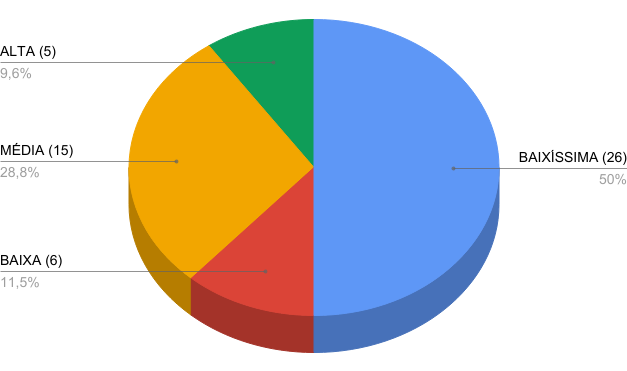
\includegraphics[width=0.45\textwidth]{grafico-recorrencia.png}
% 	\caption{Distribuição das práticas vs. recorrência}
% 	\label{fig:CategoriaXRecorrencia}
% \end{figure}

A Tabela \ref{tab:Categories} apresenta o total de ocorrências das categorias de alta, média e baixa recorrência em cada questão sobre boas e más práticas (\textit{S1}). A última linha da tabela, \#Categorias, apresenta quantas categorias emergiram de cada questão, como cada questão está diretamente ligada a um elemento do \textit{front-end} Android, podemos interpretá-la da seguinte forma: \emph{quais são os pontos de atenção a serem analisados em determinado elemento Android?} A última coluna da tabela, \#Q, apresenta em quantas questões cada categoria surgiu, podemos interpretá-la da seguinte forma: \emph{com base na categoria, quais elementos devem ser investigados?} Duas práticas, Classe Deus/Longa \cite{Riel, RefactoringFowler1999} e Herança \cite{WikipediaInhiritance}, são conceitos pré-existentes e portanto não são tratados neste artigo. 


% Quando se criam categorizações para auxiliar desenvolvedores a identificar pontos de atenção a serem avaliados e onde este pontos devem ser investigados especificamente no código, pensando em qualidade de código dá-se o nome de \textit{smells}. Portanto, nesta seção iremos compilar este conjunto de Android \textit{code smells} que identificamos através das categorizações.


\begin{table*}
\centering
\footnotesize
\begin{tabular}{@{}p{3.5cm}p{0.3cm}p{.2cm}p{.2cm}p{.2cm}p{.2cm}p{.2cm}p{.2cm}p{.2cm}p{.2cm}p{.2cm}p{.4cm}p{.4cm}p{.4cm}p{.4cm}p{.4cm}p{.4cm}p{.4cm}p{.4cm}p{.4cm}p{0.2cm}@{}}
\toprule
\textbf{Recorrência/Prática} & \multicolumn{1}{c}{\textbf{\#T}} & Q1 & Q2 & Q3 & Q4 & Q5 & Q6 & Q7 & Q8 & Q9 & Q10 & Q11 & Q12 & Q13 & Q14 & Q15 & Q16 & Q17 & Q18 &  \multicolumn{1}{c}{\textbf{\#Q}} \\
\hline
\multicolumn{2}{l}{\scriptsize{\textbf{ALTA RECORRÊNCIA (4)}}} \\
Lógica Em Classes de UI					& \multicolumn{1}{c}{60} 	& \multicolumn{1}{c}{14} 	& \multicolumn{1}{c}{15} 	& \multicolumn{1}{c}{8}		& \multicolumn{1}{c}{8}		& \multicolumn{1}{c}{6}		& \multicolumn{1}{c}{8}		& \multicolumn{1}{c}{--}	& \multicolumn{1}{c}{1}		& \multicolumn{1}{c}{--}	& \multicolumn{1}{c}{--}	& \multicolumn{1}{c}{--}	& \multicolumn{1}{c}{--}	& \multicolumn{1}{c}{--}	& \multicolumn{1}{c}{--}	& \multicolumn{1}{c}{--}	& \multicolumn{1}{c}{--}	& \multicolumn{1}{c}{--} 	& \multicolumn{1}{c}{--}	& \multicolumn{1}{c}{7} \\
Nome de Recurso Despadronizado		& \multicolumn{1}{c}{24} 	& \multicolumn{1}{c}{1} 	& \multicolumn{1}{c}{--} 	& \multicolumn{1}{c}{--}	& \multicolumn{1}{c}{--}	& \multicolumn{1}{c}{--}	& \multicolumn{1}{c}{--}	& \multicolumn{1}{c}{--}	& \multicolumn{1}{c}{--}	& \multicolumn{1}{c}{3}		& \multicolumn{1}{c}{2}		& \multicolumn{1}{c}{3}		& \multicolumn{1}{c}{2}		& \multicolumn{1}{c}{8}		& \multicolumn{1}{c}{2}		& \multicolumn{1}{c}{3}		& \multicolumn{1}{c}{--}	& \multicolumn{1}{c}{--} 	& \multicolumn{1}{c}{--}	& \multicolumn{1}{c}{8} \\
Recurso Mágico				& \multicolumn{1}{c}{23} 	& \multicolumn{1}{c}{--} 	& \multicolumn{1}{c}{--} 	& \multicolumn{1}{c}{--}	& \multicolumn{1}{c}{--}	& \multicolumn{1}{c}{--}	& \multicolumn{1}{c}{--}	& \multicolumn{1}{c}{--}	& \multicolumn{1}{c}{--}	& \multicolumn{1}{c}{4}		& \multicolumn{1}{c}{2}		& \multicolumn{1}{c}{1}		& \multicolumn{1}{c}{1}		& \multicolumn{1}{c}{9}		& \multicolumn{1}{c}{6}		& \multicolumn{1}{c}{--}	& \multicolumn{1}{c}{--}	& \multicolumn{1}{c}{--} 	& \multicolumn{1}{c}{--}	& \multicolumn{1}{c}{6} \\
Layout Profundamente Aninhado					& \multicolumn{1}{c}{21} 	& \multicolumn{1}{c}{--} 	& \multicolumn{1}{c}{--} 	& \multicolumn{1}{c}{--}	& \multicolumn{1}{c}{--}	& \multicolumn{1}{c}{1}		& \multicolumn{1}{c}{--}	& \multicolumn{1}{c}{--}	& \multicolumn{1}{c}{--}	& \multicolumn{1}{c}{9}		& \multicolumn{1}{c}{9}		& \multicolumn{1}{c}{--}	& \multicolumn{1}{c}{--}	& \multicolumn{1}{c}{--}	& \multicolumn{1}{c}{--}	& \multicolumn{1}{c}{--}	& \multicolumn{1}{c}{--}	& \multicolumn{1}{c}{1} 	& \multicolumn{1}{c}{1}		& \multicolumn{1}{c}{5} \\

\vspace{1sp} \\
\multicolumn{2}{l}{\scriptsize{\textbf{MÉDIA RECORRÊNCIA (15)}}} \\ 
Classes de UI Acopladas			& \multicolumn{1}{c}{18} 	& \multicolumn{1}{c}{--} 	& \multicolumn{1}{c}{2} 	& \multicolumn{1}{c}{4}	 	& \multicolumn{1}{c}{6} 	& \multicolumn{1}{c}{--} 	& \multicolumn{1}{c}{3} 	& \multicolumn{1}{c}{1} 	& \multicolumn{1}{c}{2} 	& \multicolumn{1}{c}{--} 	& \multicolumn{1}{c}{--} 	& \multicolumn{1}{c}{--} 	& \multicolumn{1}{c}{--} 	& \multicolumn{1}{c}{--} 	& \multicolumn{1}{c}{--} 	& \multicolumn{1}{c}{--}	& \multicolumn{1}{c}{--} 	& \multicolumn{1}{c}{--} 	& \multicolumn{1}{c}{--} 	& \multicolumn{1}{c}{6} \\
Comportamento Suspeito			& \multicolumn{1}{c}{18} 	& \multicolumn{1}{c}{2} 	& \multicolumn{1}{c}{2} 	& \multicolumn{1}{c}{--} 	& \multicolumn{1}{c}{--} 	& \multicolumn{1}{c}{1} 	& \multicolumn{1}{c}{2} 	& \multicolumn{1}{c}{7} 	& \multicolumn{1}{c}{3} 	& \multicolumn{1}{c}{--} 	& \multicolumn{1}{c}{--} 	& \multicolumn{1}{c}{--} 	& \multicolumn{1}{c}{--} 	& \multicolumn{1}{c}{--} 	& \multicolumn{1}{c}{--} 	& \multicolumn{1}{c}{--}	& \multicolumn{1}{c}{--} 	& \multicolumn{1}{c}{1} 	& \multicolumn{1}{c}{--} 	& \multicolumn{1}{c}{4} \\
Mau Uso do Ciclo de Vida					& \multicolumn{1}{c}{15} 	& \multicolumn{1}{c}{4} 	& \multicolumn{1}{c}{3} 	& \multicolumn{1}{c}{3}	 	& \multicolumn{1}{c}{5} 	& \multicolumn{1}{c}{--} 	& \multicolumn{1}{c}{--} 	& \multicolumn{1}{c}{--} 	& \multicolumn{1}{c}{--} 	& \multicolumn{1}{c}{--} 	& \multicolumn{1}{c}{--} 	& \multicolumn{1}{c}{--} 	& \multicolumn{1}{c}{--} 	& \multicolumn{1}{c}{--} 	& \multicolumn{1}{c}{--} 	& \multicolumn{1}{c}{--}	& \multicolumn{1}{c}{--} 	& \multicolumn{1}{c}{--} 	& \multicolumn{1}{c}{--} 	& \multicolumn{1}{c}{5} \\
Layout Longo ou Repetido						& \multicolumn{1}{c}{15} 	& \multicolumn{1}{c}{--} 	& \multicolumn{1}{c}{--} 	& \multicolumn{1}{c}{--} 	& \multicolumn{1}{c}{--} 	& \multicolumn{1}{c}{--} 	& \multicolumn{1}{c}{--} 	& \multicolumn{1}{c}{--} 	& \multicolumn{1}{c}{--} 	& \multicolumn{1}{c}{12} 	& \multicolumn{1}{c}{2} 	& \multicolumn{1}{c}{--} 	& \multicolumn{1}{c}{--} 	& \multicolumn{1}{c}{--} 	& \multicolumn{1}{c}{--} 	& \multicolumn{1}{c}{--}	& \multicolumn{1}{c}{--} 	& \multicolumn{1}{c}{1} 	& \multicolumn{1}{c}{--} 	& \multicolumn{1}{c}{3} \\
Não Uso de Padrão View Holder				& \multicolumn{1}{c}{13} 	& \multicolumn{1}{c}{--} 	& \multicolumn{1}{c}{--} 	& \multicolumn{1}{c}{--} 	& \multicolumn{1}{c}{--} 	& \multicolumn{1}{c}{11} 	& \multicolumn{1}{c}{2} 	& \multicolumn{1}{c}{--} 	& \multicolumn{1}{c}{--} 	& \multicolumn{1}{c}{--} 	& \multicolumn{1}{c}{--} 	& \multicolumn{1}{c}{--} 	& \multicolumn{1}{c}{--} 	& \multicolumn{1}{c}{--} 	& \multicolumn{1}{c}{--} 	& \multicolumn{1}{c}{--}	& \multicolumn{1}{c}{--} 	& \multicolumn{1}{c}{--} 	& \multicolumn{1}{c}{--} 	& \multicolumn{1}{c}{2} \\
Classe Deus/Longa*				& \multicolumn{1}{c}{13} 	& \multicolumn{1}{c}{2} 	& \multicolumn{1}{c}{4} 	& \multicolumn{1}{c}{2}	 	& \multicolumn{1}{c}{2} 	& \multicolumn{1}{c}{--} 	& \multicolumn{1}{c}{1} 	& \multicolumn{1}{c}{--} 	& \multicolumn{1}{c}{1} 	& \multicolumn{1}{c}{--} 	& \multicolumn{1}{c}{--} 	& \multicolumn{1}{c}{--} 	& \multicolumn{1}{c}{1} 	& \multicolumn{1}{c}{--} 	& \multicolumn{1}{c}{--} 	& \multicolumn{1}{c}{--}	& \multicolumn{1}{c}{--} 	& \multicolumn{1}{c}{--} 	& \multicolumn{1}{c}{--} 	& \multicolumn{1}{c}{6} \\
Não Uso de Arquiteturas Conhecidas		& \multicolumn{1}{c}{13} 	& \multicolumn{1}{c}{4} 	& \multicolumn{1}{c}{--} 	& \multicolumn{1}{c}{2}	 	& \multicolumn{1}{c}{--} 	& \multicolumn{1}{c}{--} 	& \multicolumn{1}{c}{--} 	& \multicolumn{1}{c}{--} 	& \multicolumn{1}{c}{--} 	& \multicolumn{1}{c}{--} 	& \multicolumn{1}{c}{--} 	& \multicolumn{1}{c}{--} 	& \multicolumn{1}{c}{--} 	& \multicolumn{1}{c}{--} 	& \multicolumn{1}{c}{--} 	& \multicolumn{1}{c}{--}	& \multicolumn{1}{c}{--} 	& \multicolumn{1}{c}{6} 	& \multicolumn{1}{c}{1} 	& \multicolumn{1}{c}{4} \\
Tamanho Único de Imagem		& \multicolumn{1}{c}{12} 	& \multicolumn{1}{c}{--} 	& \multicolumn{1}{c}{--} 	& \multicolumn{1}{c}{--} 	& \multicolumn{1}{c}{--} 	& \multicolumn{1}{c}{--} 	& \multicolumn{1}{c}{--} 	& \multicolumn{1}{c}{--} 	& \multicolumn{1}{c}{--} 	& \multicolumn{1}{c}{1} 	& \multicolumn{1}{c}{1} 	& \multicolumn{1}{c}{--} 	& \multicolumn{1}{c}{--} 	& \multicolumn{1}{c}{--} 	& \multicolumn{1}{c}{--} 	& \multicolumn{1}{c}{4}		& \multicolumn{1}{c}{6} 	& \multicolumn{1}{c}{--} 	& \multicolumn{1}{c}{--} 	& \multicolumn{1}{c}{7} \\
Uso Excessivo de Fragment	& \multicolumn{1}{c}{11} 	& \multicolumn{1}{c}{--} 	& \multicolumn{1}{c}{--} 	& \multicolumn{1}{c}{8}	 	& \multicolumn{1}{c}{3} 	& \multicolumn{1}{c}{--} 	& \multicolumn{1}{c}{--} 	& \multicolumn{1}{c}{--} 	& \multicolumn{1}{c}{--} 	& \multicolumn{1}{c}{--} 	& \multicolumn{1}{c}{--} 	& \multicolumn{1}{c}{--} 	& \multicolumn{1}{c}{--} 	& \multicolumn{1}{c}{--} 	& \multicolumn{1}{c}{--} 	& \multicolumn{1}{c}{--}	& \multicolumn{1}{c}{--} 	& \multicolumn{1}{c}{--} 	& \multicolumn{1}{c}{--} 	& \multicolumn{1}{c}{4} \\
Não Uso de Imagens Vetoriais			& \multicolumn{1}{c}{10} 	& \multicolumn{1}{c}{--} 	& \multicolumn{1}{c}{--} 	& \multicolumn{1}{c}{--} 	& \multicolumn{1}{c}{--} 	& \multicolumn{1}{c}{--} 	& \multicolumn{1}{c}{--} 	& \multicolumn{1}{c}{--} 	& \multicolumn{1}{c}{--} 	& \multicolumn{1}{c}{--} 	& \multicolumn{1}{c}{--} 	& \multicolumn{1}{c}{--} 	& \multicolumn{1}{c}{--} 	& \multicolumn{1}{c}{--} 	& \multicolumn{1}{c}{--} 	& \multicolumn{1}{c}{10}	& \multicolumn{1}{c}{--} 	& \multicolumn{1}{c}{--} 	& \multicolumn{1}{c}{--} 	& \multicolumn{1}{c}{1} \\
Não Uso de Fragment					& \multicolumn{1}{c}{9} 	& \multicolumn{1}{c}{3} 	& \multicolumn{1}{c}{2} 	& \multicolumn{1}{c}{4}	 	& \multicolumn{1}{c}{--} 	& \multicolumn{1}{c}{--} 	& \multicolumn{1}{c}{--} 	& \multicolumn{1}{c}{--} 	& \multicolumn{1}{c}{--} 	& \multicolumn{1}{c}{--} 	& \multicolumn{1}{c}{--} 	& \multicolumn{1}{c}{--} 	& \multicolumn{1}{c}{--} 	& \multicolumn{1}{c}{--} 	& \multicolumn{1}{c}{--} 	& \multicolumn{1}{c}{--}	& \multicolumn{1}{c}{--} 	& \multicolumn{1}{c}{--} 	& \multicolumn{1}{c}{--} 	& \multicolumn{1}{c}{2} \\
Classes de UI Fazendo IO					& \multicolumn{1}{c}{9} 	& \multicolumn{1}{c}{1} 	& \multicolumn{1}{c}{4} 	& \multicolumn{1}{c}{1}	 	& \multicolumn{1}{c}{2} 	& \multicolumn{1}{c}{--} 	& \multicolumn{1}{c}{1} 	& \multicolumn{1}{c}{--} 	& \multicolumn{1}{c}{--} 	& \multicolumn{1}{c}{--} 	& \multicolumn{1}{c}{--} 	& \multicolumn{1}{c}{--} 	& \multicolumn{1}{c}{--} 	& \multicolumn{1}{c}{--} 	& \multicolumn{1}{c}{--} 	& \multicolumn{1}{c}{--}	& \multicolumn{1}{c}{--} 	& \multicolumn{1}{c}{--} 	& \multicolumn{1}{c}{--} 	& \multicolumn{1}{c}{4} \\
Longo Recurso de Estilo			& \multicolumn{1}{c}{8} 	& \multicolumn{1}{c}{--} 	& \multicolumn{1}{c}{--} 	& \multicolumn{1}{c}{--} 	& \multicolumn{1}{c}{--} 	& \multicolumn{1}{c}{--} 	& \multicolumn{1}{c}{--} 	& \multicolumn{1}{c}{--} 	& \multicolumn{1}{c}{--} 	& \multicolumn{1}{c}{--} 	& \multicolumn{1}{c}{--} 	& \multicolumn{1}{c}{5} 	& \multicolumn{1}{c}{3} 	& \multicolumn{1}{c}{--} 	& \multicolumn{1}{c}{--} 	& \multicolumn{1}{c}{--}	& \multicolumn{1}{c}{--} 	& \multicolumn{1}{c}{--} 	& \multicolumn{1}{c}{--} 	& \multicolumn{1}{c}{2} \\
Recurso de String Bagunçado	& \multicolumn{1}{c}{8} 	& \multicolumn{1}{c}{--} 	& \multicolumn{1}{c}{--} 	& \multicolumn{1}{c}{--} 	& \multicolumn{1}{c}{--} 	& \multicolumn{1}{c}{--} 	& \multicolumn{1}{c}{--} 	& \multicolumn{1}{c}{--} 	& \multicolumn{1}{c}{--} 	& \multicolumn{1}{c}{--} 	& \multicolumn{1}{c}{--} 	& \multicolumn{1}{c}{--} 	& \multicolumn{1}{c}{--} 	& \multicolumn{1}{c}{4} 	& \multicolumn{1}{c}{4} 	& \multicolumn{1}{c}{--}	& \multicolumn{1}{c}{--} 	& \multicolumn{1}{c}{--} 	& \multicolumn{1}{c}{--} 	& \multicolumn{1}{c}{2} \\
Atributos de Estilo Repetidos	& \multicolumn{1}{c}{8} 	& \multicolumn{1}{c}{--} 	& \multicolumn{1}{c}{--} 	& \multicolumn{1}{c}{--} 	& \multicolumn{1}{c}{--} 	& \multicolumn{1}{c}{--} 	& \multicolumn{1}{c}{--} 	& \multicolumn{1}{c}{--} 	& \multicolumn{1}{c}{--} 	& \multicolumn{1}{c}{1} 	& \multicolumn{1}{c}{2} 	& \multicolumn{1}{c}{2} 	& \multicolumn{1}{c}{2} 	& \multicolumn{1}{c}{--} 	& \multicolumn{1}{c}{--} 	& \multicolumn{1}{c}{--}	& \multicolumn{1}{c}{--} 	& \multicolumn{1}{c}{1} 	& \multicolumn{1}{c}{--} 	& \multicolumn{1}{c}{5} \\

\vspace*{1sp} \\
\multicolumn{2}{l}{\scriptsize{\textbf{BAIXA RECORRÊNCIA (6)}}} \\
Activity Inexistente			& \multicolumn{1}{c}{7}  	& \multicolumn{1}{c}{2}  	& \multicolumn{1}{c}{4}  	& \multicolumn{1}{c}{--} 	& \multicolumn{1}{c}{--} 	& \multicolumn{1}{c}{--} 	& \multicolumn{1}{c}{--} 	& \multicolumn{1}{c}{--} 	& \multicolumn{1}{c}{1} 	& \multicolumn{1}{c}{--} 	& \multicolumn{1}{c}{--} 	& \multicolumn{1}{c}{--} 	& \multicolumn{1}{c}{--} 	& \multicolumn{1}{c}{--} 	& \multicolumn{1}{c}{--} 	& \multicolumn{1}{c}{--} 	& \multicolumn{1}{c}{--} 	& \multicolumn{1}{c}{--} 	& \multicolumn{1}{c}{--} 	& \multicolumn{1}{c}{3} \\
Imagem Dispensável					& \multicolumn{1}{c}{6}  	& \multicolumn{1}{c}{--}  	& \multicolumn{1}{c}{--}  	& \multicolumn{1}{c}{--} 	& \multicolumn{1}{c}{--} 	& \multicolumn{1}{c}{--} 	& \multicolumn{1}{c}{--} 	& \multicolumn{1}{c}{--} 	& \multicolumn{1}{c}{--} 	& \multicolumn{1}{c}{1} 	& \multicolumn{1}{c}{--} 	& \multicolumn{1}{c}{--} 	& \multicolumn{1}{c}{--} 	& \multicolumn{1}{c}{--} 	& \multicolumn{1}{c}{--} 	& \multicolumn{1}{c}{3} 	& \multicolumn{1}{c}{2} 	& \multicolumn{1}{c}{--} 	& \multicolumn{1}{c}{--} 	& \multicolumn{1}{c}{3} \\
Excessivo Reúso de String		& \multicolumn{1}{c}{6}  	& \multicolumn{1}{c}{--}  	& \multicolumn{1}{c}{--}  	& \multicolumn{1}{c}{--} 	& \multicolumn{1}{c}{--} 	& \multicolumn{1}{c}{--} 	& \multicolumn{1}{c}{--} 	& \multicolumn{1}{c}{--} 	& \multicolumn{1}{c}{--} 	& \multicolumn{1}{c}{--} 	& \multicolumn{1}{c}{--} 	& \multicolumn{1}{c}{--} 	& \multicolumn{1}{c}{--} 	& \multicolumn{1}{c}{2} 	& \multicolumn{1}{c}{4} 	& \multicolumn{1}{c}{--} 	& \multicolumn{1}{c}{--} 	& \multicolumn{1}{c}{--} 	& \multicolumn{1}{c}{--} 	& \multicolumn{1}{c}{4} \\
Adapter Complexo				& \multicolumn{1}{c}{6}  	& \multicolumn{1}{c}{--}  	& \multicolumn{1}{c}{--}  	& \multicolumn{1}{c}{--} 	& \multicolumn{1}{c}{--} 	& \multicolumn{1}{c}{3} 	& \multicolumn{1}{c}{2} 	& \multicolumn{1}{c}{--} 	& \multicolumn{1}{c}{--} 	& \multicolumn{1}{c}{--} 	& \multicolumn{1}{c}{1} 	& \multicolumn{1}{c}{--} 	& \multicolumn{1}{c}{--} 	& \multicolumn{1}{c}{--} 	& \multicolumn{1}{c}{--} 	& \multicolumn{1}{c}{--} 	& \multicolumn{1}{c}{--} 	& \multicolumn{1}{c}{--} 	& \multicolumn{1}{c}{--} 	& \multicolumn{1}{c}{2} \\
Herança**						& \multicolumn{1}{c}{5}  	& \multicolumn{1}{c}{2}  	& \multicolumn{1}{c}{--}  	& \multicolumn{1}{c}{2} 	& \multicolumn{1}{c}{--} 	& \multicolumn{1}{c}{1} 	& \multicolumn{1}{c}{--} 	& \multicolumn{1}{c}{--} 	& \multicolumn{1}{c}{--} 	& \multicolumn{1}{c}{--} 	& \multicolumn{1}{c}{--} 	& \multicolumn{1}{c}{--} 	& \multicolumn{1}{c}{--} 	& \multicolumn{1}{c}{--} 	& \multicolumn{1}{c}{--} 	& \multicolumn{1}{c}{--} 	& \multicolumn{1}{c}{--} 	& \multicolumn{1}{c}{--} 	& \multicolumn{1}{c}{--} 	& \multicolumn{1}{c}{3} \\
Listener Escondido				& \multicolumn{1}{c}{5}  	& \multicolumn{1}{c}{--}  	& \multicolumn{1}{c}{--}  	& \multicolumn{1}{c}{--} 	& \multicolumn{1}{c}{--} 	& \multicolumn{1}{c}{--} 	& \multicolumn{1}{c}{--} 	& \multicolumn{1}{c}{2} 	& \multicolumn{1}{c}{3} 	& \multicolumn{1}{c}{--} 	& \multicolumn{1}{c}{--} 	& \multicolumn{1}{c}{--} 	& \multicolumn{1}{c}{--} 	& \multicolumn{1}{c}{--} 	& \multicolumn{1}{c}{--} 	& \multicolumn{1}{c}{--} 	& \multicolumn{1}{c}{--} 	& \multicolumn{1}{c}{--} 	& \multicolumn{1}{c}{--} 	& \multicolumn{1}{c}{3} \\
\hline
\multicolumn{2}{r}{\textbf{\#Totais}} 		& \multicolumn{1}{c}{35} & \multicolumn{1}{c}{36} & \multicolumn{1}{c}{34} & \multicolumn{1}{c}{26} & \multicolumn{1}{c}{23} & \multicolumn{1}{c}{19} & \multicolumn{1}{c}{10} & \multicolumn{1}{c}{11} & \multicolumn{1}{c}{31} & \multicolumn{1}{c}{19} & \multicolumn{1}{c}{11} & \multicolumn{1}{c}{9} & \multicolumn{1}{c}{23} & \multicolumn{1}{c}{16} & \multicolumn{1}{c}{20} & \multicolumn{1}{c}{8} & \multicolumn{1}{c}{10} & \multicolumn{1}{c}{2} \\
\hline
\multicolumn{2}{r}{\textbf{\#Categorias}} 	& \multicolumn{1}{c}{10} & \multicolumn{1}{c}{8} & \multicolumn{1}{c}{9} & \multicolumn{1}{c}{6} & \multicolumn{1}{c}{6} & \multicolumn{1}{c}{7} & \multicolumn{1}{c}{3} & \multicolumn{1}{c}{6} & \multicolumn{1}{c}{7} & \multicolumn{1}{c}{7} & \multicolumn{1}{c}{4} & \multicolumn{1}{c}{5} & \multicolumn{1}{c}{4} & \multicolumn{1}{c}{4} & \multicolumn{1}{c}{4} & \multicolumn{1}{c}{2} & \multicolumn{1}{c}{5} & \multicolumn{1}{c}{2} \\
\hline
% \multicolumn{20}{@{}l@{}}{* Classe Deus \cite{Riel} e Classe Longa \cite{RefactoringFowler1999} são \textit{code smells} tradicionais previamente definidos em literaturas. ** Herança é um conceito da Programação Orientada a Objetos \cite{WikipediaInhiritance}. \textbf{\#T}: recorrência geral da categoria. \textbf{\#Q}: total de questões distintas em cada categoria. A linha \textbf{\#Totais}: total de respostas obtidas em cada questão. \textbf{\#Categorias}: total de categorias distinstas de cada questão.} \\

\multicolumn{20}{@{}l}{* Classe Deus \cite{Riel} e Classe Longa \cite{RefactoringFowler1999} são cheiros de código tradicionais previamente definidos em literaturas.} \\
\multicolumn{20}{@{}l}{** Herança é um conceito da Programação Orientada a Objetos \cite{WikipediaInhiritance}.} \\
\multicolumn{20}{@{}l}{Coluna \textbf{\#T}: recorrência geral da prática.} \\
\multicolumn{20}{@{}l}{Coluna \textbf{\#Q}: total de questões distintas por prática.} \\
\multicolumn{20}{@{}l}{Linha \textbf{\#Totais}: total de respostas obtidas em cada questão.} \\
\multicolumn{20}{@{}l}{Linha \textbf{\#Categorias}: total de categorias distinstas de cada questão.} \\
\toprule
\end{tabular}
\caption{Lista de práticas de alta, média e baixa recorrência.}
\label{tab:Categories}
\end{table*}

Esta Seção está organizada em 4 subseções onde, nas três primeiras, definimos as práticas de alta, média e baixa recorrência, \emph{totalizando 23 más práticas}. Na última subseção apresentamos os resultados obtidos no estudo sobre a percepção de desenvolvedores com relação às más práticas de alta recorrência. As práticas de baixíssima recorrência são brevemente discutidas na Seção \ref{discussao}.

% ----------------------- ALTA RECORRÊNCIA -----------------------
\subsection{Más Práticas de Alta Recorrência}
% Obtivemos 4 categorias consideradas de alta recorrência: Lógica Em Classes de UI, Nome de Recurso Despadronizado, Recurso Mágico e Layout Profundamente Aninhado.

\subsubsection{Lógica Em Classes de UI (LCUI)}
Indicam como má prática haver regras de negócio nos elementos como \textsc{Activities}, \textsc{Fragments}, \textsc{Listeners} e \textsc{Adapters} e indicam como boas práticas que esses mesmos elementos contenham apenas códigos relacionados a interface com o usuário. Para isso sugerem o uso de padrões como: \textit{Model-View-Presenter} (MVP) \cite{MartinFowlerGUIArchitectures, WikipediaMVP}, \textit{Model-View-ViewModel} (MVVM) \cite{WikipediaMVVM} e \textit{Clean Architecture} \cite{CleanArchitecture}. Exemplos de frases que indicaram más práticas são: P16 sobre \textsc{Activities} diz \textit{``Fazer lógica de negócio''} (tradução livre)\footnote{Todo texto em inglês foi traduzido livremente ao longo do artigo.}, P19 diz \textit{``Colocar regra de negócio no adapter''} e P11 diz \textit{``Manter lógica de negócio em Fragments''}. Exemplos de frases que indicaram boas prática são: P16 diz \textit{``Elas [\textsc{Activities}] representam uma única tela e apenas interagem com a UI, qualquer lógica deve ser delegada para outra classe''}, P23 diz \textit{``Apenas código relacionado à Interface de Usuário nas Activities''}, P40 diz \textit{``Adapters devem apenas se preocupar sobre como mostrar os dados, sem trabalhá-los''}, P2 diz \textit{``As activities que eu crio normalmente tem um propósito único e estado básico [...] eu uso MVP a maior parte do tempo, então minhas activities normalmente representam uma view no MVP''}. Os elementos afetados por essa categoria são: \textsc{Activities}, \textsc{Fragments}, \textsc{Listeners} e \textsc{Adapters}. 

\subsubsection{Nome de Recurso Despadronizado (NRD)}
Indicam como má prática o não uso de um padrão de nomenclatura a ser usado nos recursos da aplicação. De forma similar, respostas indicam como boas práticas o uso de um padrão de nomenclatura a ser usados nos recursos. Exemplos de frases que indicaram más práticas são: P8 sobre \textsc{Style Resources} diz \textit{``[...] o nome das strings sem um contexto''}, P37 também sobre \textsc{Style Resources} diz \textit{``Nada além de ter uma boa convenção de nomes''}, ainda P37, porém sobre \textsc{Layout Resources} diz \textit{``Mantenha uma convenção de nomes da sua escolha [...]''}. Exemplos de frases que indicaram boas prática são: P27 diz sobre \textsc{String Resources} \textit{``Iniciar o nome de uma string com o nome da tela onde vai ser usada''}, P43 sobre \textsc{Layout Resources} diz \textit{``Ter uma boa convenção de nomeação''}, P11 diz sobre \textsc{Style Resources} \textit{``[...] colocar um bom nome [...]''}. Os elementos que entraram nessa categoria foram: \textsc{Activities}, \textsc{Layout Resources}, \textsc{String Resources}, \textsc{Style Resources} e \textsc{Drawable Resources}. 

Dentre as respostas, algumas indicaram padrões de preferência. P11 indica usar prefixos nos \textsc{Layout Resources}: \texttt{activity\_}, \texttt{fragment\_}, \texttt{ui\_} (para UI customizadas). P12 sugeriu usar sufixos em \textsc{Activities}: \texttt{\_Activity}. Os padrões indicados para \textsc{String Resources} foram: P27 indicou \textit{``Iniciar o nome da string com o nome da tela onde vai ser usada''}, P6 sugeriu a convenção \texttt{[screen]\_[type]\_[text]} e citou como exemplo \texttt{welcome\_message\_title}. P34 indicou que deve-se usar como prefixo o recurso usando a string, por exemplo \texttt{dialog.STRING\_NAME} ou \texttt{hint.STRING\_NAME}. De forma similar porém sem sugerir um exemplo, P4 sugeriu basear o nome da string no nome do recurso que a esta usando. Não foram sugeridos nenhum padrão para \textsc{Styles Resources} e \textsc{Drawable Resources}.

\subsubsection{Recurso Mágico (RM)}
Indicam como má prática o uso direto de valores como, por exemplo, strings, números e cores, sem a criação um recurso. De forma similar, respostas indicam como boas práticas o uso de um padrão de nomenclatura a ser usados nos recursos. O nome dessa categoria foi inspirado no cheiro de código \textit{Magic Number} \cite{Martin:2008:CCH:1388398} que trata sobre números usados diretamente no código. Exemplos de frases que indicaram más práticas são: P23 diz \textit{``Strings diretamente no código''}, P31 e P35 falam respectivamente sobre não extrair as strings e sobre não extrair os valores dos arquivos de layout. Exemplos de frases que indicaram boas prática são: P7 diz \textit{``Sempre pegar valores de string ou dp de seus respectivos resources para facilitar''}, P36 diz para \textit{``sempre adicionar as strings em resources para traduzir em diversos idiomas [...]''}. Os elementos que entraram nessa categoria foram: \textsc{Layout Resources}, \textsc{String Resources} e \textsc{Style Resources}. 


\subsubsection{Layout Profundamente Aninhado (LPA)} 
Indicam como má prática o uso de profundos aninhamentos na construção de layouts. De forma similar, respostas indicam como boas práticas evitar ao máximo o aninhamento de \textit{views}. Exemplos de frases que indicaram más práticas são: P26 diz \textit{``Hierarquia de views longas''}, P4 aborda a mesma ideia ao dizer \textit{``Estruturas profundamente aninhadas''}, P39 diz \textit{``Hierarquias desnecessárias''} e P45 diz \textit{``Criar muitos ViewGroups dentro de ViewGroups''}. Exemplos de frases que indicaram boas prática são: P4 diz \textit{``tento usar o mínimo de layout aninhado''}, P19 diz \textit{``Utilizar o mínimo de camadas possível''}, P8 diz \textit{``[...] não fazer uma hierarquia profunda de ViewGroups [...]''}. Apenas o elemento \textsc{Layout Resources} recebeu esta categoria. O site oficial do Android conta com informações e ferramentas automatizadas para lidar com esse sintoma \cite{OptmizingViewHierarchies}. 


% ----------------------- MÉDIA RECORRÊNCIA -----------------------
\subsection{Más Práticas de Média Recorrência}
% Obtivemos 15 práticas consideradas de média recorrência. Dentre elas, duas representam uma prática de orientação a objetos (herança) e um cheiro de código já conhecido (Classe Deus/Longa), essas duas, não são definidas a seguir.

\subsubsection{Classes de UI Acopladas (CUIA)}
Indicam como má prática o acoplamento entre \textsc{Activities}, \textsc{Fragments}, \textsc{Adapters} e \textsc{Listeners}, ou seja, a existência de referências diretas entre elas. De forma similar, respostas indicam como boas práticas que estas classes não se conheçam diretamente. Com base nas respostas, identificamos 3 situações onde essa má prática é percebida.

O primeira situação é quando o \textsc{Fragment} está acoplado à \textsc{Activities}, outros \textsc{Fragments} ou componentes. Sobre o acoplamento de \textsc{Fragments} com \textsc{Activities}, P19 diz \textit{``Acoplar o fragment a activity ao invés de utilizar interfaces é uma prática ruim''}. P10, P31 e P45 indicam como má prática \textit{``acoplar o \textsc{Fragment} com a \textsc{Activity}''}. Sobre o acoplamento de \textsc{Fragments} com outros \textsc{Fragments}, P37 diz que \textit{``Fragments nunca devem tentar falar uns com os outros diretamente''} e P45 diz \textit{``[é uma má prática] integragir com outro Fragment diretamente''}. Sobre o \textsc{Fragments} serem acoplados a outros componentes, P6 diz \textit{``Seja um componente de UI reutilizável. Então evite dependência de outros componentes da aplicação''}. Como boa prática, para a comunicação entre essas classes, são indicados: o uso de \textit{interfaces}, o método \textsc{onAttach} existente em \textsc{Fragments} (este método é disparado pelo Android ao associar um \textsc{Fragment} a uma \textsc{Activity}) ou a biblioteca \textit{EventBus} \cite{EventBusAndroid}. P36 diz \textit{``Criar uma interface para a comunicação entre Activity e Fragment, ou utilizar o EventBus.''} e P44 diz \textit{``Use e abuse do método onAttach para se comunicar com Activity''}. 

A segunda situação é quando o \textsc{Listener} está acoplado à \textsc{Activities}. P40 diz que é uma má prática \textit{``[o \textsc{Listener}] conter uma referência forte à Activities''}, P4 exprime a mesma ideia com uma frase um pouco diferente. 

A terceira situação é quando o \textsc{Adapter} está acoplado à \textsc{Activities} ou \textsc{Fragments}. P10 indicou como má prática em \textit{Adapters} o \textit{``alto acoplamento com a Activity''} e P45 exprime a mesma ideia ao dizer \textit{``Acessar Activities ou Fragments diretamente''}. 

% Os elementos que entraram nessa categoria foram: \textsc{Activities}, \textsc{Fragments}, \textsc{Listeners} e \textsc{Adapters}. 

\subsubsection{Comportamento Suspeito (CS)}
Indicam boas e más práticas ao implementar comportamento para responder a eventos do usuário, como por exemplo, um toque na tela. Um evento do usuário é representado através de \textsc{listeners}, que são interfaces Java onde cada uma representa um tipo de evento, por exemplo, a interface \texttt{OnClickListener} representa o evento de clique. Através das respostas dos participantes identificamos como boas práticas o uso de classes concretas e ferramentas de injeção de eventos e como más práticas o uso de classes an\^onimas e classes internas.

Classes an\^onimas são consideradas como má prática por todos os participantes que comentaram sobre ela, onde a maioria sugeriu o uso de classes concretas. Por exemplo, P9 diz \textit{``Usar muitos an\^onimos pode ser complicado. Às vezes nomear coisas torna mais fácil para depuração''}, P4 diz \textit{``Mantenha-os [listeners] em classes separadas (esqueça sobre classes an\^onimas)''}, P32 diz \textit{``Prefiro declarar os listeners com "implements" e sobrescrever os métodos (onClick, por exemplo) do que fazer um set listener no próprio objeto''} e P8 diz \textit{``Muitas implementações de listener com classes an\^onimas''}.

O uso de classes internas também foi considerado como má prática. Exemplos de frases que indicam más práticas são: P42 diz \textit{``Declarar como classe interna da Activity ou Fragment ou outro componente que contém um ciclo de vida. Isso pode fazer com que os aplicativos causem vazamentos de memória.''}.

O polimorfismo, fazendo com que o elemento Android implemente o \textsc{Listener}, foi considerado uma má prática por alguns participantes, esses sugeriram o uso de classes concretas ou de ferramentas de injeção de eventos e dependência como \textit{Butter Knife} \cite{ButterKnife} e \textit{Dagger2}. Por exemplo: P44 diz \textit{``Eu não gosto quando os desenvolvedores fazem a activity implementar o listener porque eles [os métodos] serão expostos e qualquer um pode chamá-lo de fora da classe. Eu prefiro instanciar ou então usar ButterKnife para injetar cliques.''}. P6 diz \textit{``Tome cuidade se a activity/fragment é um listener uma vez que eles são destruídos quando as configurações mudam. Isso causa vazamentos de memória.''}, P10 diz \textit{``Use carregamento automático de view como ButterKnife e injeção de dependência como Dagger2''}. Para outros, esta forma de implementação é uma boa prática, por exemplo P32 diz \textit{``Prefiro declarar os listeners com "implements" e sobrescrever os métodos (onClick, por exemplo) do que fazer um set listener no próprio objeto.''}.

Os elementos que entraram nesta categoria foram: \textsc{Activity}, \textsc{Fragment} ou \textsc{Adapter}.

\subsubsection{Mau Uso do Ciclo de Vida (MUCV)}
Indicam como má prática o uso incorreto do ciclo de vida \textsc{Activities} e \textsc{Fragments}. De forma similar, respostas indicam como boas práticas respeitar o ciclo de vida desses elementos e não confundir o ciclo de vida de ambos. Exemplos de frases que indicaram más práticas são: P23 diz \textit{``código que depende de estado e não se adapta ao ciclo de vida das Activities.''}, P28 diz \textit{``Erros ao interpretar o ciclo de vida''}, P8 diz \textit{``considerar o ciclo de vida de fragments como os de activities''}. Exemplos de frases que indicaram boas prática são: P43 diz \textit{``Conhecer seu [da activity] ciclo de vida''}, P28, P31 e P15 falam \textit{``tomar cuidado e respeitar o ciclo de vida de \textsc{fragments} e \textsc{activities}''}. Os elementos que entraram nessa categoria foram: \textsc{Activities} e \textsc{Fragments}. 

\subsubsection{Layout Longo ou Repetido (LLR)}
Indicam como má prática código de \textit{layout} repetido ou muito grandes. De forma similar, respostas indicam como boas práticas extrair layout repetidos para reutilizá-los através da tag \textsc{include} ou extrair apenas com o objetivo de manter arquivos pequenos. Exemplos de frases que indicaram más práticas são: P41 diz \textit{``copiar e colar layouts parecidos sem usar includes''}, P23 diz \textit{``[...] colocar muitos recursos no mesmo arquivo de layout.''}, P8 diz \textit{``considerar o ciclo de vida de fragments como os de activities''}. Exemplos de frases que indicaram boas prática são: P32 diz \textit{``Sempre quando posso, estou utilizando includes para algum pedaço de layout semelhante''}, P36diz \textit{``Criar layouts que possam ser reutilizados em diversas partes''} e P42 diz \textit{``Separe um grande layout usando include ou merge''}. 


\subsubsection{Longos Recursos de Layout (LRL)}
Indicam como má prática arquivos \textsc{Layout Resources} grandes e complexos. Respostas indicam como boas práticas a quebra desses arquivos em vários outros e o uso da \textit{tag} de layout \texttt{include} para uni-los. Exemplos de frases que indicaram más práticas são: P41 diz \textit{``Copiar e colar trechos similares de tela, sem usar includes''}, P23 diz \textit{``[...] utilizar muitos recursos no mesmo arquivo de layout''}. Exemplos de frases que indicaram boas prática são: P34 diz \textit{``eu apenas tento reusá-los através do uso de includes''}, P40 diz \textit{``modularize-os''}, P9 diz \textit{use includes para simplificar multiplas configurações [de tela]}. 

\subsubsection{Não Uso de Padrão View Holder (MUVH)}
Indicam como má prática o não uso do padrão \textit{View Holder} \cite{AluraViewHolder} para melhorar o desempenho de listagens. De forma similar, respostas indicam como boas práticas evitar o uso do padrão \textit{View Holder}. Exemplo de frase que indicou má prática é P8 ao dizer \textit{``[...] evitar o padrão ViewHolder''}. Exemplos de frases que indicaram boas prática são: P36 diz \textit{``Reutilizar a view utilizando ViewHolder.''}, de forma similar P39 diz \textit{``Usar o padrão ViewHolder''}. P45 sugere o uso do \textsc{RecyclerView}, um elemento Android para a construção de listas que já implementa o padrão \textit{ViewHolder} \cite{AluraViewHolder}. Apenas o elemento \textsc{Adapter} entrou nessa categoria. 

\subsubsection{Não Uso de Arquiteturas Conhecidas (NUAC)}
Indicam como má prática o não uso de algum padrão para desacoplar código de apresentação com código de lógica. De forma similar, respostas indicam como boas práticas o uso de algum padrão conhecido e sugerem MVP, MVC, MVVM e Clen Architecture. Exemplos de frases que indicaram más práticas são: P45 diz \textit{``Sobre não usar um design pattern''}. Exemplos de frases que indicaram boas prática são: P28 diz \textit{``Usar algum modelo de arquitetura para garantir apresentação desacoplada do framework (MVP, MVVM, Clean Architecture, etc)''}, P45 diz \textit{``Sobre MVP. Eu acho que é o melhor padrão de projeto para usar com Android''}. Os elementos que entraram nessa categoria foram: \textsc{Activities} e textsc{Fragments}. 

\subsubsection{Tamanho Único de Imagem (TUI)}
Indicam como má prática ter apenas uma imagem para atender a todas as resoluções. De forma similar, respostas indicam como boas práticas ter a mesma imagem em diversos tamanhos para atender a resoluções diferentes. Exemplos de frases que indicaram más práticas são: P31 diz \textit{``ter apenas uma imagem para multiplas densidades''}, P4 diz \textit{``Baixar uma imagem muito grande quando não é necessário. Há melhores formas de usar memória''}, P44 diz \textit{``Não criar [versões da] imagem para todos as resoluções''}. Exemplos de frases que indicaram boas prática são: P34 diz \textit{``Nada especial, apenas mantê-las em seus respectivos diretórios e ter variados tamanhos delas''}, P36 diz \textit{``Criar as pastas para diversas resoluções e colocar as imagens corretas''}. O único elemento que entrou nessa categoria é o que representa imagens, \textsc{Drawable Resource}.

\subsubsection{Uso Excessivo de Fragment (UEF)}
Indicam como má prática o uso de \textsc{Fragments} quando se pode usar \textsc{Activities} e o uso excessivo de \textsc{Fragments}. De forma similar, respostas indicam como boas práticas evitar o uso de \textsc{Fragments} sempre que possível. Exemplos de frases que indicaram más práticas são: P2 diz \textit{``Usar muitos Fragments é uma má prática''}. Exemplos de frases que indicaram boas prática são: P16 diz \textit{``Eu tento evitá-los''}. Os elementos que entraram nessa categoria foram: \textsc{Fragments}. 

\subsubsection{Não Uso de Imagens Vetoriais (NUIV)}
I10 participantes) que indicam como boa prática o uso de \textsc{Drawable Resources} vetoriais. é recomendado sempre que possível usar imagens vetorias sobre outros tipos. Exemplos de frases que indicaram boas prática são: P28 diz \textit{``Utilizar o máximo de Vector Drawables que for possível''}, P40 diz \textit{``evite muitas imagens, use imagens vetoriais sempre que possível''}. O único elemento que entrou nessa categoria é o que representa imagens, \textsc{Drawable Resource}.

\subsubsection{Não Uso de Fragment (NUF)}
Indicam como má prática o não uso de \textsc{Fragments}. De forma similar, respostas indicam como boas práticas o uso de \textsc{Fragments} sempre que possível. Exemplos de frases que indicaram más práticas são: P22 diz \textit{``Não usar Fragments''}. Exemplos de frases que indicaram boas prática são: P19 diz \textit{``[...] Utilizar fragments sempre que possível.''}, P45 diz \textit{``Use Fragments para cada tela. Uma Activity para cada app/apk.''}. Os elementos que entraram nessa categoria foram: \textsc{Fragments} e \textsc{Activities}. \mau{como esse se relaciona com o 2 acima dele?}

\subsubsection{Classes de UI Fazendo IO (CUIFIO)}
Indicam como má prática realizar operações de IO, como consulta a banco de dados ou acesso a internet, a partir das classes \textsc{Activities}, \textsc{Fragments} e \textsc{Adapters}. Respostas indicam como boas práticas que esses elementos lidem apenas com a interface com o usuário e sugerem para isso, o padrão MVP \cite{WikipediaMVP, MartinFowlerGUIArchitectures}. Exemplos de frases que indicaram más práticas são: P26 sobre \textsc{Activities} e \textsc{Fragments} diz \textit{``fazer requests e consultas a banco de dados''} e sobre \textsc{Adapter} diz \textit{``Fazer operações longas e requests de internet''}. P37 sobre \textsc{Activities} diz \textit{``Elas nunca devem fazer acesso a dados [...]''}. Exemplos de frases que indicaram boas prática são: P26 diz \textit{``Fazer activities e fragments apenas lidar com ações da view, faça isso usando o [padrão] MVP''}. Os elementos que entraram nessa categoria foram: \textsc{Activities}, \textsc{Fragments} e \textsc{Adapters}. 

\subsubsection{Longo Recurso de Estilo (LRE)}
Indicam como má prática o uso de apenas um arquivo para todos os \textsc{Styles Resources}. De forma similar, respostas indicam como boas práticas separar os estilos em mais de um arquio. Exemplos de frases que indicaram más práticas são: P28 diz \textit{``Deixar tudo no mesmo arquivo styles.xml''}, P8 diz \textit{``Arquivos de estilos grandes''}. Exemplos de frases que indicaram boas prática são: P28 diz \textit{``Se possível, separar mais além do arquivo styles.xml padrão, já que é possível declarar múltiplos arquivos XML de estilo para a mesma configuração''}. P40 diz \textit{``Divida-os. Temas e estilos é uma escolha racional''}. O único elemento que entrou nessa categoria foi o \textsc{Style Resource}. 

\subsubsection{Recurso de String Bagunçado (RSB)}
Indicam como má prática arquivos \textsc{String Resources} desorganizados ou o uso de apenas um arquivo para todos os \textsc{String Resources}. De forma similar, respostas indicam como boas práticas separar as \textit{strings} em mais de um arquivo. Exemplos de frases que indicaram más práticas são: P28 diz \textit{``Usar o mesmo arquivo strings.xml para tudo''}, P42 diz \textit{``Não orgaizar as strings quando o strings.xml começa a ficar grande''}. Exemplos de frases que indicaram boas prática são: P28 diz \textit{``Separar strings por tela em arquivos XML separados. Extremamente útil para identificar quais strings pertencentes a quais telas em projetos grandes''}. P32 diz \textit{``Sempre busco separar em blocos, cada bloco representa uma activity e nunca aproveito uma String pra outra tela''}. O único elemento que entrou nessa categoria foi o \textsc{String Resource}. 

\subsubsection{Atributos de Estilo Repetidos (AER)}
Indicam como má prática a repetição de atributos de estilo nos \textsc{Layout Resource}. De forma similar, respostas indicam como boas práticas sempre que identificar atributos repetidos, extraí-los para um estilo. Exemplos de frases que indicaram más práticas são: P32 diz \textit{``Utilizar muitas propriedades em um único componente. Se tiver que usar muitas, prefiro colocar no arquivo de styles.''}. Exemplos de frases que indicaram boas prática são: P34 diz \textit{``Sempre que eu noto que tenho mais de um recurso usando o mesmo estilo, eu tento movê-lo para o meu \textit{style resource}.''}. Os elementos nessa categoria foram: \textsc{Layout Resources} e \textsc{Style Resources}.



% ----------------------- BAIXA RECORRÊNCIA -----------------------
\subsection{Más Práticas de Baixa Recorrência}
% Obtivemos 8 categorias consideradas de baixa recorrência: Imagem Dispensável, Activity Inexistente, Ferramentas de DI, Excessivo Reúso de String, Adapter Flexível, Operações de IO, Herança e Listener Escondido.


\subsubsection{Activity Inexistente (AI)}
Indicam como má prática classes manterem referência a uma \textsc{Activity}, pois como ela possui ciclo de vida, quando a classe tentar acessá-la, a \textsc{Activity} pode não existir mais, resultando em possíveis erros na aplicação. De forma similar, respostas indicam como boas práticas, elementos com ciclo de vida independente, não manter referência à \textsc{Activities}. Exemplos de frases que indicaram más práticas são: P28 diz \textit{``Fazer Activities serem callbacks de processos assíncronos gerando memory leaks. Erros ao interpretar o ciclo de vida''}, P31 diz \textit{``[...] ter referência estática para Activities, resultando em vazamento de memória''}. Exemplos de frases que indicaram boas prática são: P31 diz \textit{``Não manter referências estáticas para Activities (ou classes an\^onimas criadas dentro delas)''}, P4 diz \textit{``Deus mata um cachorro toda vez que alguém passa o contexto da Activity para um componente que tem um ciclo de vida independente dela. Vaza memória e deixa todos tristes.''}. Os elementos que entraram nessa categoria foram: \textsc{Activities} e \textsc{Listeners}. 

\subsubsection{Imagem Dispensável (ID)}
Indicam como má prática o uso de imagens quando poderia ser usado um \textsc{Drawable Resource} em XML. De forma similar, respostas indicam como boas práticas o uso de \textsc{Drawable Resources}, criado com XML, sempre que possível. Exemplos de frases que indicaram más práticas são: P23 diz \textit{``Uso de formatos não otimizados, uso de drawables onde recursos padrão do Android seriam preferíveis''}, P37 diz \textit{usar jpg ou png para formas simples é ruim, apenas as desenhe [através de \textsc{Drawable Resources}]}. Exemplo de frase que indicou boa prática é P36 que diz \textit{``[...] Quando possível, criar resources através de xml.''}. Apenas o elemento \textsc{Drawable Resoirce} entrou nessa categoria. 

\subsubsection{Excessivo Reúso de String (ERS)}
Indicam como má prática reutilizar o mesmo \textsc{String Resource} em muitos lugares no aplicativo, apenas porque o texto coincice, pois caso seja necessário alterar em um lugar, todos os outros serão afetados. De forma similar, respostas indicam como boas práticas considerar a semântica ou contexto ao nomear um \textsc{String Resource}, para mesmo que o valor seja o mesmo, os recursos sejam diferentes. Exemplos de frases que indicaram más práticas são: P32 diz \textit{``Utilizar uma String pra mais de uma activity, pois se em algum momento, surja a necessidade de trocar em uma, vai afetar outra.''}, P6 diz \textit{``Reutilizar a string em várias telas''} e P40 diz \textit{``Reutilizar a string apenas porque o texto coincide, tenha cuidado com a semântica''}. Exemplos de frases que indicaram boas prática são: P32 diz \textit{``Sempre busco separar em blocos, cada bloco representa uma activity e nunca aproveito uma String pra outra tela.''} e P9 diz \textit{``Não tenha medo de repetir strings [...]''}. Apenas o elemento \textsc{String Resource} entrou nessa categoria. 

\subsubsection{Adapter Complexo (AC)}
Indicam como má prática \textsc{Adapters} que contém muitos condicionais. Respostas indicam como boas práticas que um \textsc{Adapter} deve adaptar apenas um tipo de classe e trabalhar com um ou mais views, de forma a evitar lógicas para esconder ou mostrar view expecíficas. Exemplos de frases que indicaram más práticas são: P23 diz \textit{``Reutilizar um mesmo adapter para várias situações diferentes, com "ifs" ou "switches". Código de lógica importante ou cálculos em Adapters.''}. Exemplos de frases que indicaram boas prática são: P2 diz \textit{``Um Adapter deve adaptar um único tipo de item ou delegar a Adapters especializados''}. O único elemento que entrou nessa categoria foi o \textsc{Adapter}. 

\subsubsection{Listener Escondido (LE)}
Indicam como má prática o uso de métodos de eventos do usuário no XML de layout, como por exemplo o método \textsc{onClick}. Respostas indicam como boas práticas o uso da biblioteca \textit{ButterKnife} \cite{ButterKnife}. Exemplos de frases que indicaram más práticas são: P34 diz \textit{``Nunca crie um listener dentro do XML. Isso esconde o listener de outros desenvolvedores e pode causar problemas até que ele seja encontrado''}, P39 e P41 expressam a mesma opinião, P41 ainda complementa dizendo que \textit{``XML de layout deve lidar apenas com a view e não com ações''}. Exemplos de frases que indicaram boas prática são: P39 diz apenas \textit{``Uso ButterKnife''}, P34 também expressa sua preferência por essa biblioteca. Apenas \textsc{Listeners} entraram nessa categoria.



% \subsection{Categorias de Baixíssima Recorrência}
% Obtivemos 29 categorias consideradas de baixíssima recorrência: MVC, Clean Architecture, Don't Use Fragment, Nested Fragment, Mix String Resources With Business Logic, Use 9 Patch Files, Dealing With App Stack Manually, Styles Knows Too Much, Package Structure, MVVM, Activity Handle More Than One Layout, Bad Relative, Deprecated Attributes, Fat onCreate, HTML Into String File, Inherit From Support Library Always, Listener Has A Valid Context, Safe Adapter, Single Activity, Static Things On Adapter, Style Into String File, Use Constraint Layout, Dead Resources, DRY, SOLID, Reuse, Singleton, Opened Activity e Unnecessary ViewGroup








% -*- root: article.tex -*-
\subsection{Percepção dos Desenvolvedores}

\begin{figure*}
\centering
\begin{subfigure}{.22\textwidth}
  \centering
  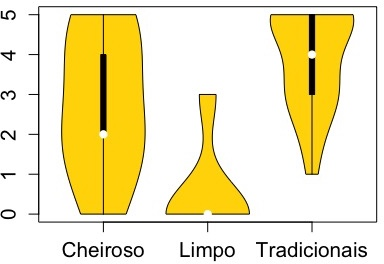
\includegraphics[width=1\textwidth]{plot-lcui-violin3.jpg}
  \caption{LCUI}
  \label{fig:lcui}
\end{subfigure}%
\begin{subfigure}{.17\textwidth}
  \centering
  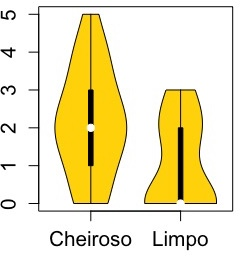
\includegraphics[width=.85\textwidth]{plot-recursos-violin2.jpg}
  \caption{Integrados}
  \label{fig:resources}
\end{subfigure}%
\begin{subfigure}{.17\textwidth}
  \centering
  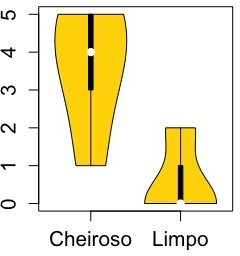
\includegraphics[width=.85\textwidth]{plot-lpa-violin2.jpg}
  \caption{LPA}
  \label{fig:lpa}
\end{subfigure}% 
\begin{subfigure}{.17\textwidth}
  \centering
  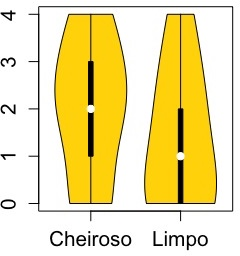
\includegraphics[width=.85\textwidth]{plot-rm-violin.jpg}
  \caption{RM}
  \label{fig:rm}
\end{subfigure}
\begin{subfigure}{.17\textwidth}
  \centering
  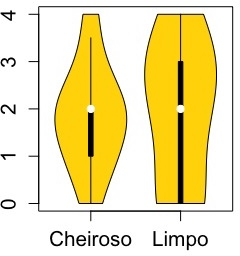
\includegraphics[width=.85\textwidth]{plot-nrd-violin.jpg}
  \caption{NRD}
  \label{fig:nrd}
\end{subfigure}% 
\caption{Gráficos violino individuais das más práticas que afetam recursos (LPA, RM e NRD).}
\label{fig:all-resources}
\vspace{-.5cm} 
\end{figure*}


As Figuras \ref{fig:lcui} e \ref{fig:all-resources} apresentam gráficos de violino sobre a percepção dos desenvolvedores com relação as quatro más práticas de alta recorrência (LCUI, LPA, RM e NRD). 

No eixo y, 0 (zero) indica códigos não percebidos pelos desenvolvedores como problemáticos (ou seja, responder \emph{não} à pergunta: este código apresenta algum problema de design e/ou implementação?), enquanto que valores de 1 a 5 indicam o nível de severidade para o problema percebido pelo desenvolvedor.

\subsubsection{Más práticas que afetam classes Java}
% \begin{figure}
% 	\centering
% 	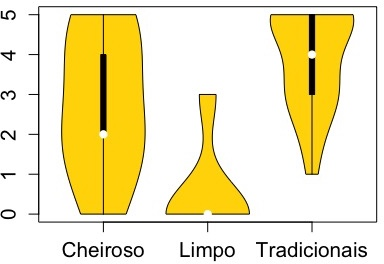
\includegraphics[width=0.3\textwidth]{plot-lcui-violin3.jpg}
% 	\caption{LCUI}
% 	\label{fig:lcui}
% \end{figure}

Na Figura \ref{fig:lcui} apresentamos três gráficos violinos, respectivamente: percepção dos desenvolvedores sobre códigos afetados pela má prática LCUI, a percepção sobre códigos limpos e por último, a percepção sobre códigos afetados por maus cheiros tradicionais como por exemplo Classe Longa. 

A mediana de classes limpas tem severidade igual a 0 (Q3=0). Isso indica que, como esperado, desenvolvedores não percebem essas classes como problemáticas. Em comparação, as classes afetadas por LCUI tem mediana igual a 2 (Q3=4) logo, são percebidas como classes problemáticas. A diferença entre classes afetadas por LCUI e classes limpas é estatisticamente significante (p-value < 0.004) com alto tamanho de efeito (d = 0,72). Com relação aos maus cheiros tradicionais, a mediana de severidade é igual a 4 (Q3=5). Isso significa que classes afetadas por esses maus cheiros são percebidas pelos desennvolvedores como muito problemáticas, ainda mais que classes afetadas pela má prática em questão. Ainda que essa diferença de percepção esteja clara no gráfico violino, esta diferença não é estatisticamente significante (p-value = 0.077). Acreditamos que isso ocorra devido ao número limitado de dados (20 participantes).

% LCIU p-value e d completos/originais/sem quebrar decimal
% Notamos que, desenvolvedores de fato percebem classes afetadas pela má prática LCUI como problemáticas (p-value 0.003045 e d 0.7222222 (large)). Bem como, classes afetadas por maus cheiros tradicionais também são percebidas como problemáticas (p-value 6.367e-06 e d -0.9130435 (large)). Porém, não podemos afirmar se, maus cheiros tradicionais são considerados mais ou menos importantes do que a má prática LCUI (p-value 0.07667 e d -0.3961353 (medium)). Ao observar as respostas abertas, a maioria dos participantes pontuou a questão de haver lógica na classe de \textit{front-end}, que é o ponto central desta má prática, como o problema. Podemos citar S2P11 que diz ``\textit{[...] Não há nenhuma arquitetura implementada, o que causa a classe fazendo muito mais do que é de sua alçada. O método onListItemClick está muito complexo, contendo 7 condições [...]}''.

\subsubsection{Más práticas que afetam recursos}

A Figura \ref{fig:all-resources} reúne 4 diferentes pares de gráficos violinos. O primeiro compara recusos afetados por quaisquer das 3 más práticas, LPA, RM e NRD, com recursos limpos. O segundo, terceiro e quarto, trata de cada má prática individualmente, ou seja, recursos afetadas por aquela má prática em comparação com recursos limpos. 

A Figura \ref{fig:resources} mostra a percepção dos desenvolvedores com relação a recursos afetados pelas más práticas LPA, RND e RM, com mediana de severidade igual a 2 (Q3=3), em comparação com recursos limpos (mediana igual a 0). Isso indica que, como esperado, desenvolvedores percebem recursos afetados pelas más práticas como problemáticos. Essa diferença também é estatisticamente significante (p-value < 0.008) com médio tamanho de efeito (d = 0.43).

% XMLS vs LIMPOS dados completos
% podemos observar que, de fato, desenvolvedores percebem, de forma geral, recursos afetados pelas más práticas LPA, RM ou NRD, como problemáticos (p-value 0.007986 e $\delta$ 0.4335664 (medium)). 

Ao avaliarmos os gráficos violinos das más práticas individualmente, podemos notar que duas, LPA (Figura \ref{fig:lpa}) e RM (Figura \ref{fig:rm}), se mostram percebidas como problemáticas, sendo a primeira mais percebida do que a segunda. Códigos afetados pela má prática LPA tem mediana de severidade igual a 4 (Q3=5) logo, desenvolvedores percebem códigos afetados por ela como problemáticos. Em comparação, código limpos apresentam mediana 0 (Q3=1). A diferença entre códigos afetados por LPA e códigos limpos também é estatisticamente significante (p-value < 0.02) com alto tamanho de efeito (d = 0,89). Em contrapartida, ainda que o gráfico de violino da má prática RM apresente também uma diferença visual entre códigos limpos e afetados pela má prática, essa diferença não é estatisticamente significante (p-value = 0,34).

A má prática NRD foi a menos percebida por desenvolvedores, com medianas iguais para códigos afetados por ela e códigos limpos (mediana = 2). Entretando, os desenvolvedores que indicaram códigos afetados por ela como problemáticos, indicaram como o problema descrições muito próximas a definição dada para essa má prática. Por exemplo, S2P15 disse ``\textit{Os nomes das strings são formados por um prefixo e um número, o que prejudica a legibilidade, é impossível saber o que este número indica}'' (pontuou severiadade como 3), S2P16 disse ``\textit{Atributos não seguem convenção de nomes. Nomes não são descritivos}'' (pontuou severiadade como 2), S2P11 disse ``\textit{Não segue uma boa prática de nomenclatura de recursos.}'' (pontuou severiadade como 2) e S2P19 disse ``\textit{Os nomes das strings não estão seguindo um padrão (algumas em camelCase, outras lowercase, outras snakecase) [...]}'' (pontuou severiadade como 2). Algumas possíveis ideias que justificariam esse resultado são discutidas na Seção \ref{discussao}. \\

De forma geral, os desenvolvedores conseguiram identificar corretamente a má prática em questão, colocando em suas respostas descrições muito próximas as definições dadas a elas. Por exemplo S2P11 ao confrontar um código afetado por LCUI disse ``\textit{[...] Não há nenhuma arquitetura implementada, o que causa a classe fazendo muito mais do que é de sua alçada. O método onListItemClick está muito complexo, contendo 7 condições [...]}'', S2P5 ao confrontar um código afetado por RM disse ``\textit{Valores de cores, tamanhos, animaçoes e distancias, nao estao extraidos fazendo que muitos deles estejam repetidos dificultando uma posterior manutençao ou reusabilidade}'', S2P7 ao confrontar um código afetado por LPA disse ``\textit{Os sucessivos aninhamentos de view groups provavelmente irá causar uma performance ruim}''.

% \begin{figure*}
% \centering
% \begin{subfigure}{.19\textwidth}
%   \centering
%   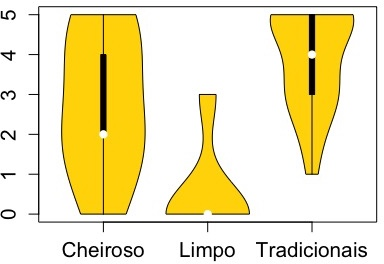
\includegraphics[width=1.1\textwidth]{plot-lcui-violin3.jpg}
%   \caption{LCUI}
%   \label{fig:lcui}
% \end{subfigure}%
% \begin{subfigure}{.19\textwidth}
%   \centering
%   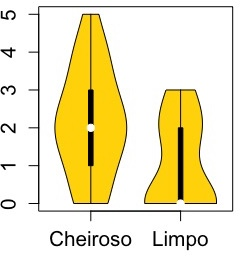
\includegraphics[width=.7\textwidth]{plot-recursos-violin2.jpg}
%   \caption{Integrados}
%   \label{fig:resources}
% \end{subfigure}%
% \begin{subfigure}{.19\textwidth}
%   \centering
%   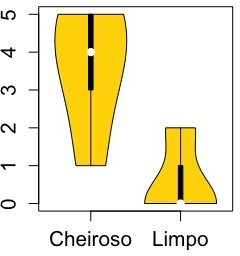
\includegraphics[width=.7\textwidth]{plot-lpa-violin2.jpg}
%   \caption{LPA}
%   \label{fig:lpa}
% \end{subfigure}% 
% \begin{subfigure}{.19\textwidth}
%   \centering
%   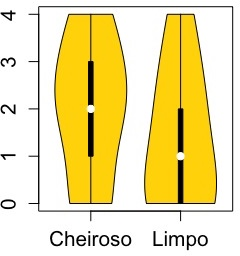
\includegraphics[width=.7\textwidth]{plot-rm-violin.jpg}
%   \caption{RM}
%   \label{fig:rm}
% \end{subfigure}
% \begin{subfigure}{.19\textwidth}
%   \centering
%   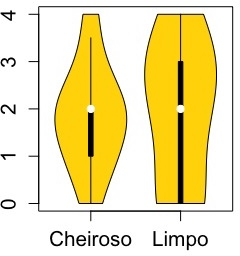
\includegraphics[width=.7\textwidth]{plot-nrd-violin.jpg}
%   \caption{NRD}
%   \label{fig:nrd}
% \end{subfigure}% 
% \caption{Gráficos violino individuais das más práticas que afetam recursos (LPA, RM e NRD).}
% \label{fig:all-resources}
% \end{figure*}













\section{Discussão}
\label{discussao}
% -*- root: article.tex -*-
% \lettrine[nindent=0em,lines=2]{L}

[Under construction] \\

% Consideramos inconclusivo se a utliza\c{c}\~ao de Fragments \'e recomendada ou n\~ao. 2 participantes afirmaram enfaticamente que n\~ao se deve usar \textsc{Fragments}, por exemplo, segundo P7, uma m\'a pr\'atica sobre \textsc{Fragments} \'e ``o uso deles''.

\section{Ameaças à Validade}
\label{ameacas}
\mau{aqui veja também o paper da michaela, para ver como se escreve ameacas em trabalhos qualitativos.}
% -*- root: article.tex -*-
Uma limitação deste artigo é que os dados foram coletados apenas a partir de questionários online e o processo de codificação foi realizado apenas por um dos autores. Alterativas a esses cenários seria realizar a coleta de dados de outras formas como entrevistas ou consulta a especialistas, e que o processo de codificação fosse feito por mais de um autor de forma a reduzir possúveis enviezamentos.

Outra possível ameaça é com relação a seleção de códigos limpos. Selecionar códigos limpos é difícil. Sentimos uma dificuldade maior ao selecionar códigos de recursos do Android. Um alternativa seria investigar a existência de ferramentas que façam esta selecão, validar os códigos selecionados com um especialista ou mesmo extender o teste piloto. 

Nossa pesquisa tenta replicar o método utilizado por Aniche \cite{FinavaroAniche2016} ao investigar cheiros de código no framework Spring MVC. Entretando, nos deparamos com situações diferentes, das quais, após a execução nos questionamos se aquele método seria o mais adequado para o contexto deste artigo. Por exemplo, nosso resultado com a má prática RM nos levou a conjecturar se desenvolvedores consideram problemas em códigos Java mais severos que problemas em recursos do aplicativo. O que nos levou a pensar sobre isso foi que, apesar do resultado, obtivemos muitas respostas que se aproximavam da deifnição da má prática RM. Desta forma, levantamos que de todos os recursos avaliados, 74\% receberam severidade igual ou inferior a 3, contra 30\% com os mesmo níveis de severidade em código Java. Desta forma, uma alternativa seja repensar a forma de avaliar a percepção dos desenvolvedores sobre más práticas que afetem recursos do aplicativo.


\section{Trabalhos Relacionados}
\label{relacionados}
% -*- root: article.tex -*-
Muitas pesquisas t\^em sido realizadas sobre a plataforma Android, muitas delas focam em vulnerabilidades \cite{Y, F, G, X, P, D, E}, autentica\c{c}\~ao \cite{T, Yamashita6405287, R} e testes \cite{J, M}. Diferentemente dessas pesquisas, nossa pesquisa tem foco na percep\c{c}\~ao dos desenvolvedores sobre boas e m\'as pr\'aicas de desenvolvimento na plataforma Android. 

A percep\c{c}\~ao desempenha um importante papel na defini\c{c}\~ao de code smells relacionados a uma tecnologia, visto que code smells possuem uma natureza subjetiva. Code smells desempenham um importante papel na busca por qualidade de c\'odigo, visto que, ap\'os mapeados, podemos chegar a heur\'isticas para identific\'a-los e com essas heur\'isticas, implementar ferramentas que automatizem o processo de identificar c\'odigos problem\'aticos.

Verloop \cite{MobileSmells:13} conduziu um estudo no qual avaliou por meio de 4 ferramentas de detec\c{c}\~ao automatizada de cheiros de c\'odigo (JDeodorant, Checkstyle, PMD e UCDetector) a presen\c{c}a de 5 cheiros de c\'odigo (Long Method, Large Class, Long Parameter List, Feature Envy e Dead Code) em 4 projetos Android. Nossa pesquisa se relaciona com a de Verloop no sentido de que tamb\'em estamos buscando por cheiros de c\'odigo, entretanto, em vez de de buscarmos por cheiros de c\'odigo j\'a definidos, realizamos uma abordagem inversa na qual, primeiro buscamos entender a percep\c{c}\~ao de desenvolvedores sobre boas e m\'as pr\'aticas em Android, e a partir dessa percep\c{c}\~ao, relacionamos com algum cheiro de c\'odigo pr\'e-existente ou derivamos algum novo.

Gottschalk et al \cite{EnergyAndroidSmells} conduziram um estudo sobre formas de detectar e refatorar cheiros de c\'odigo relacionados ao uso efici\^ente de energia. Os autores compilaram um cat\'alogo com 8 cheiros de c\'odigo e trabalharam sob um trecho de c\'odigo Android para exemplificar um deles, o "binding resource too early", quando algum recurso \'e alocado muito antes de precisar ser utilizado. Essa pesquisa \'e relacionada \`a nossa por ambas considerarem a tecnologia Android e se diferenciam pois focamos na busca por cheiros de c\'odigo relacionados a qualidade de c\'odigo, no sentido de legibilidade e manutenablidade.

Aplicativos Android s\~ao escritos na linguagem de programa\c{c}\~ao Java \cite{AndroidFundamentals}. Ent\~ao a primeira quest\~ao \'e: por que buscar por \textit{smells} Android sendo que j\'a existem tantos \textit{smells} Java? Pesquisas t\^em demonstrado que tecnologias diferentes podem apresentar \textit{code smells} espec\'ificos, como por exemplo Aniche et al. identificaram 6 \textit{code smells} espec\'ificos ao framework Spring MVC, um framework Java para desenvolvimento web. Outras pesquisas concluem que projetos Android possuem caracter\'isticas diferentes de projetos java \cite{Hecht2015, Mannan_Dig_Ahmed_Jensen_Abdullah_Almurshed, ReimannBrylski2013}, por exemplo, o \textit{front-end} \'e representado por arquivos XML e o ponto de entrada da aplica\c{c}\~ao \'e dado por \textit{event-handler} \cite{AndroidActivities2016} como o m\'etodo \textsc{onCreate}. Encontramos tamb\'em diversas pesquisas sobre \textit{code smells} sobre tecnologias usadas no desenvolvimento de \textit{front-end} web como CSS \cite{CSSCodeSmell} e JavaScript \cite{BB}. Essas pesquisas nos inspiraram a buscar entender se existem \textit{code smells} no \textit{front-end} Android. \\


% \textbf{[se\c{c}\~ao n\~ao finalizada, \'a concluir.]}

\section{Conclusão}
\label{conclusao}
% -*- root: article.tex -*-
% \lettrine[nindent=0em,lines=2]{L}

[Under construction] \\

% Consideramos inconclusivo se a utliza\c{c}\~ao de Fragments \'e recomendada ou n\~ao. 2 participantes afirmaram enfaticamente que n\~ao se deve usar \textsc{Fragments}, por exemplo, segundo P7, uma m\'a pr\'atica sobre \textsc{Fragments} \'e ``o uso deles''.


\bibliographystyle{ACM-Reference-Format}
\bibliography{sigproc,dissertation} 

\end{document}
